\documentclass{book}
\usepackage[a4paper, margin=20mm]{geometry}
\usepackage{wrapfig}
\usepackage{amsmath}
\usepackage{svg}
\usepackage{graphicx}
\usepackage{authblk}
\usepackage{float}
\usepackage{caption}
\usepackage{subcaption}
\usepackage{tikz}
\usepackage{enumitem}
\usepackage{pifont}
\usepackage{scrhack}
\usepackage{amssymb}
\usepackage[english]{babel}
\usepackage[numbers]{natbib}
\usepackage{nomencl}
\usepackage{hyperref}
\usepackage{longtable}
\usepackage{listings}
\usepackage{enumitem}
\hypersetup{linktoc=all}
\graphicspath{{figures/}}

\usetikzlibrary{calc,patterns,decorations.pathmorphing,decorations.markings,shapes.geometric}
\setlength{\tabcolsep}{14pt}
\renewcommand{\arraystretch}{1.2}
\tikzstyle{spring}=[decorate,decoration={coil,pre length=0.2cm,post length=0.2cm,segment length=4}]
\tikzstyle{damper}=[decoration={markings,  
  mark connection node=dmp,
  mark=at position 0.5 with 
  {
    \node (dmp) [inner sep=0pt,transform shape,rotate=-90,minimum width=8pt,minimum height=3pt,draw=none] {};
    \draw ($(dmp.north east)+(2pt,0)$) -- (dmp.south east) -- (dmp.south west) -- ($(dmp.north west)+(2pt,0)$);
    \draw ($(dmp.north)+(0,-3pt)$) -- ($(dmp.north)+(0,3pt)$);
  }
}, decorate]

\begin{document}
\frontmatter

% Cover page
\begin{titlepage}
	
	\begin{minipage}[t]{0.6\textwidth}
		\textsf{Ain Shams University} \\
		\textsf{Faculty of Engineering} \\
		\textsf{Mechatronics Engineering Program} \\
		\textsf{Specialized CHEP}\\
		\begin{tikzpicture}[remember picture, overlay]
			\node[anchor=north east, inner sep=20mm] at (current page.north east)
			{
\includegraphics[scale=0.075]{asu.png}};
		\end{tikzpicture}
	\end{minipage}
	
	\vfill
	
	\vfill
	\begin{center}
		\Huge\textbf{Active Suspension System:\\ Modern Control Techniques} \\[10pt]
		\Large{BSc. Graduation Project (1)} \\[5pt]
		\Large{MCT491s}
	\end{center}
	
	\vfill
	
	% Submitted by
	\begin{center}
		\textbf{Submitted by:} \\
		\begin{tabular}{ ll }
			Abdelrahman Abdelhakim    & 2002103 \\
			Abd Elgahni Beshir		  & 2001753 \\
			Roberto Nasr Shawky       & 1902325 \\	
			
		\end{tabular} \\
	\end{center}
	
	\vfill
	
	% Supervisors
	\begin{center}
		\textbf{Supervisors:} \\
		Dr. Omar Shehata, Associate Professor \\
		Dr. Mohamed Abdelwahab, Assistant Professor \\
	    
	
	\end{center}
	
	\vfill
	
	% Submitted in
	\begin{center}
		\textbf{Submitted in:} \\
		29 January, 2025 \\
		Cairo, EGYPT
	\end{center}
	
	
\end{titlepage}

% Setup of the document
\chapter*{ACKNOWLEDGEMENTS}
First and foremost, we would like to express our deepest gratitude and heartfelt thanks to our families for their endless  support, understanding, and encouragement. Your belief in us, even during the most challenging moments and failures, has been our greatest source of motivation. This achievement would not have been possible without your love and sacrifices. To our friends and colleagues, thank you for your encouragement and shared experiences that have made this journey memorable and rewarding. We are also grateful to our college (Ain Shams University, Faculty of Engineering) for providing us with the resources and opportunity to pursue this project and achieve our academic goals. This milestone is a testament to the collective effort of everyone who stood by us, and we are forever thankful. And finally without our supervisors we would not do such an amazing work, thanks a lot.

\chapter*{ABSTRACT}
This thesis investigates the performance of various advanced control techniques applied to an active suspension system using a quarter-car model. The quarter-car model is widely used due to its simplicity and effectiveness in capturing the essential dynamics of a suspension system while allowing for efficient analysis and simulation. Simulation experiments are conducted to evaluate the effectiveness of these control algorithms.\\

The study focuses on the application of Linear Quadratic Regulator (LQR) for linear-time-invariant systems, Reinforcement Learning (RL), and Sliding Mode Control (SMC) to enhance suspension performance. LQR is particularly powerful for its ability to provide optimal control solutions by minimizing a defined cost function, balancing performance and energy efficiency. RL, on the other hand, offers a data-driven approach that adapts to system uncertainties and non-linearities, making it highly suitable for complex and dynamic environments. Additionally, the robustness of SMC makes it effective in handling system disturbances and parameter variations. Furthermore, the impact of state estimation using a Kalman filter is assessed, as it enables accurate estimation of unmeasured states, enhancing the overall control performance.\\

MATLAB/Simulink is employed to perform the simulations, beginning with the mathematical modeling of the system in state-space form, followed by the implementation of these modern control techniques. This research aims to contribute to a deeper understanding of control theory and its practical application in improving vehicle ride comfort and handling. By comparing the performance metrics of each control strategy, the study seeks to highlight the strengths and limitations of these advanced techniques, providing valuable insights into their applicability for real-world suspension systems.

\tableofcontents
\listoffigures
\listoftables

\chapter*{Nomenclature}

\begin{longtable}{lll}                                             \\
		
	\textbf{Symbol} & \textbf{Description} & \textbf{Unit} \\  
	$b_{s}$  & Damper average damping coefficient & N.s/m \\  
	$b_{tr}$ & Tire damping coefficient & N.s/m \\  
	$e$     & Signal error & - \\  
	$f$     & Frequency & Hz \\  
	$f_{n-s}$ & Sprung mass natural frequency & Hz \\  
	$f_{n-{us}}$ & Unsprung mass natural frequency & Hz \\  
	$k$     & Stiffness of the Suspension Spring & N/m \\  
	$k_{t}$ & Equivalent Spring Stiffness of the Tire & N/m \\  
	$L$     & Lenght of Conecting rod & mm \\  
	$M$     & Sprung Mass & kg \\  
	$m$     & Unsprung Mass & kg \\  
	$R$     & Lenght of Crank & mm \\  
	$S_D$   & Sprung displacment & mm \\  
	$STD$   & Static Tire Deflection & mm \\  
	$T$     & Periodic Time & s \\  
	$X$     & Position of the slider & mm \\  
	$z$     & Vertical Position of The Car Body & mm \\  
	$z_{{r}}$ & Road Excitation Displacement & m \\  
	$z_{{t}}$ & Vertical position of Unsprung Mass & m \\  
	$\theta$ & Angle of the crank & degrees \\  
	
	
	%$K_p$              & Propetional gain                                      & -             \\
	%$K_I$              & Intergration gain                             		   & -             \\
	%$K_d$              & Differential gain                 			            & -             \\

	%$N_p$              & Negative big                           				   & -             \\
	%$N_M$              & Negative medium                            			   & -             \\
	%$N_S$              & Negative small                            				  & -             \\
	%$P_S$              & Positve Small                             				 & -             \\
	%$P_M$              & Positve medium                           				   & -             \\
	%$P_B$              & Positve big                             				 & -             \\

	
	
\end{longtable}

\chapter*{Abbreviations}
\thispagestyle{plain}
\begin{flushleft}
	\begin{tabular}{ll}
		
	\textbf{Symbol} & \textbf{Description}\\	
	%AC   & Alternating Current \\
	ASS  & Active Suspension System \\
	%DC   & Direct Current \\
	DOF  & Degree-of-Freedom \\
	DTD  & Dynamic Tire Deflection \\
	EMI  & Electromagnetic Interference \\
	FA   & Actuator Force \\
	FLC  & Fuzzy Logic Control \\
	IMU  & Inertial Measurement Unit \\
	LQR  & Linear Quadratic Regulator \\
	LVDT & Linear Variable Displacement Transducer \\
	MPC  & Model Predictive Control \\
	MR   & Magnetorheological \\
	PI   & Performance Index \\
	PSS  & Passive Suspension System \\
	%PWA  & Piece-wise Affine Function \\
	RF   & Radio Frequency \\
	RL   & Reinforcement learning \\
	RMS  & Root Mean Square \\
	RPM  & Revolution per minute \\
	SD   & Sprung Mass Displacement \\
	SMC  & Sliding Mode Control \\
	ST   & Suspension Travel \\
	STD  & Static Tire Deflection \\
	%TOF  & Time-of-Flight \\
	TR   & Transmissibility Ratio \\
	UD   & Unsprung Mass Displacement \\
	%VFD  & Variable Frequency Drive \\
	%VSS  & Variable Structure Systems \\
	    %FDM  & Fused Deposition Modeling \\
		%NMPC & Nonlinear Model Predictive Control \\
		%eMPC & Explicit Model Predictive Control \\
		
		
		
	\end{tabular}
\end{flushleft}

\mainmatter
\chapter{Introduction}
This chapter provides an introduction to vehicle suspension systems, outlining their fundamental characteristics and components. It begins by exploring various methods of classifying suspension systems and offers an overview of the terminology commonly used in suspension system technology. Detailed descriptions are included for several prevalent suspension components. It is important to highlight that this project specifically focuses on a prepared vertical test rig simulating a quarter-car model, which serves as the foundation for our study and analysis of suspension systems. 


\section{Importance of Suspension System}
Suspension components, particularly spring, as the system elastic member, and damper have a profound effect as it serve a dual purpose contributing to the vehicle's handling and increasing the vehicle safety and improve the level of comfort of the passengers and keeping vehicle occupants comfortable and reasonably well isolated from road noise, bumps, and vibrations (better overall driving experience). It is important for the suspension to keep the vehicle wheel in contact with the road surface as much as possible, because all the forces acting on the vehicle do so through the contact patches of the tires. The suspension also helps protect the vehicle itself and any cargo or luggage from damage and wear. \cite{barton2018automotive}

\section{Suspension system components}

This section provides brief overview of the essential components of suspension system, specifically springs and dampers, both of which have a profound effect on ride and handling performance. \cite{happian-smith2001introduction}

\subsection{SPRING (Elastic member)}
The suspension system incorporates an elastic link between the tires and the vehicle's body, enabling it to simultaneously press the tires onto the road surface to follow dips and absorb shocks or overloads. This system minimizes the transmission of impacts to the vehicle frame, ensuring both stability and comfort. There are three main types of springs commonly used in suspension systems: torsion bars, coil springs, and leaf springs.
	\begin{itemize}
		\item \textbf{Coil springs} are essentially wound torsion bars, prized for their exceptional endurance, compact design, and ease of mounting.
		\item \textbf{Leaf springs} consist of long, thin members that are loaded in bending. They are typically assembled using multiple thin metal layers to achieve the desired spring rate. Beyond providing suspension, they also function as linkage and damping elements.
		\item \textbf{Torsion bars} rely on the twisting motion of a long bar to provide a spring rate that reduces shock loading on the vehicle. However, their placement across the lower portion of the car makes them more difficult to package compared to other types. \cite{trzesniowski2023suspension} 
	\end{itemize}
Characteristics of spring is detailed in Appendix 1.

\subsection{DAMPER (Energy dissipation member)}
As a car passes over a bump, the springs deflect and then rebound. Without a mechanism to dissipate the energy stored in the springs, the car would continue to bounce up and down. Dampers, or shock absorbers, fulfill this critical role. A damper consists of a piston and a cylinder equipped with adjustable valves that control the flow of hydraulic fluid (oil). These valves regulate the damping force during both the retraction (bounce) and extension (rebound) phases. The damper allows oil to flow through one-way valves in the piston and small control passages from one chamber to another, but this flow is deliberately restricted, causing it to move very slowly.

This controlled fluid movement slows down the spring's oscillations, helping the car return to a stable, level ride. The damper converts the kinetic energy from the vehicle's bounce into thermal energy, effectively dissipating it. Dampers are designed to retract under a lower force than is required for extension. This asymmetry allows them to absorb road bump forces while effectively dampening spring oscillations, resulting in improved ride comfort, vehicle stability, and control. \cite{barton2018automotive}\\

\section{Suspension System Performance}
The performance of an automotive suspension system refers to how well it functions in terms of providing balance between passenger comfort, vehicle stability during all driving conditions.

Suspension dynamic performance:
	\begin{itemize}[label= ]
		\item \textbf{Vehicle Handling:} Vehicle stability and road holding (i.e. providing grip for the driver of the vehicle to control direction).
		\item \textbf{Ride Quality:} Passenger's comfort or discomfort during movement of the vehicle.	
	\end{itemize}
	
The preferred performance of a suspension system is defined by its ability to seamlessly blend vehicle handling and roadholding, evaluated through dynamic tire deflection (DTD), with ride quality assessed via the transmissibility ratio (TR). An ideal suspension system ensures that passengers enjoy a smooth and comfortable ride, free from excessive body vibrations, while also providing the driver with optimal control, stability, and responsiveness under various driving conditions.
	
A well-designed suspension system strikes the perfect balance, delivering a luxurious ride for everyday driving and dynamic handling for sporty driving. It excels in vibration isolation by effectively dampening road-induced disturbances and offers sufficient suspension travel and dynamic tire deflection to adapt to diverse terrains.
	
Performance characteristics are detailed in Appendix 2.
	
\section{Effect of suspension Parameters}
Achieving both a luxurious ride and dynamic handling for sport driving presents a significant challenge in passive suspension systems (PSS). This is due to the opposing suspension characteristics required to fulfill these two objectives simultaneously. The inherent trade-offs in automotive passive suspension systems result in compromises between comfort and performance.	
Explanation of these trade-offs is detailed in Appendix 3.
	
\section{Motivation}
The experience of oscillations during vehicle motion is a well-documented challenge that arises primarily due to irregularities and stimuli encountered on road surfaces. These oscillations have far-reaching implications, affecting passenger comfort, cargo stability, and vehicle durability. To mitigate these effects, suspension systems are engineered to regulate and attenuate oscillations, ensuring that they remain within acceptable limits.

Automotive suspension systems have evolved significantly, encompassing various designs such as passive (mechanical), semi-active, active, and pneumatic systems. Passive suspension systems, characterized by their simplicity and cost-effectiveness, dominate the market and are commonly integrated into mass-produced vehicles. They typically consist of components such as coil springs, leaf springs, torsion bars, dampers, lever arms, and stabilizer bars. While these systems perform adequately under standard conditions, their inherent limitations—such as fixed properties and lack of adaptability to dynamic external stimuli—can compromise ride comfort, particularly in challenging driving environments. To address these shortcomings, advancements in suspension technology have introduced systems with enhanced adaptability. Air suspension systems, for instance, employ air springs capable of modulating stiffness through internal pressure adjustments, offering improved responsiveness to varying road conditions. Semi-active systems, incorporating technologies like magnetorheological (MR) dampers, provide another layer of adaptability, enabling the system to better respond to road-induced oscillations.

Active suspension systems represent the pinnacle of suspension technology, capable of dynamically adjusting to changing road conditions in real-time. By actively controlling the forces applied to the suspension components, these systems offer unparalleled performance in mitigating oscillations, ensuring optimal ride comfort, and maintaining vehicle stability. This thesis aims to explore and further develop control strategies for active suspension systems, emphasizing their potential to redefine vehicle dynamics and enhance overall driving experiences. In active suspension system, a hydraulic actuator (or electromagnetic actuator) generates an impact force acting on both masses of the vehicle, gradually diminishing the vehicle's oscillation.\cite{nguyen2023design}


\section{Scope and Objective}
The main focus of this study is to perform a comparative analysis for the most commonly used modern control techniques, including LQR, SMC, and RL. The evaluation will focus on their effectiveness in reducing vertical acceleration and displacement of the sprung mass, and the suspension travel. The pros and cons of each technique will be assessed based on these results.
	
\begin{itemize}
	\item \textbf{Objectives:}
	\begin{itemize}
		\item Conducting various simulations using MATLAB/SIMULINK on the quarter car model to understand its behavior.
		\item Compare between the response of the PSS and ASS for various road profiles
		\item Implement the selected control algorithms on MATLAB/SIMULINK environment for different conditions.
		\item Conduct comparative analysis to determine the suitable control algorithm for which case.
		
	\end{itemize}
\end{itemize}	

\section{Limitations}
\begin{itemize}
\item Simplified Model: The use of a quarter-car model represents a simplification of the actual vehicle dynamics. A full-vehicle model would provide a more accurate representation of real-world behavior, considering interactions between different axles and body motions.
\item Limited Scope: The research focuses on a limited set of control strategies (LQR, RL, and SMC). Exploring other advanced control techniques, such as adaptive control and predictive control, could provide further insights into optimal suspension performance.
\item Simulation-Based: The study relies entirely on simulations. Experimental validation on a physical test rig would be necessary to further validate the findings and assess the practical feasibility of the proposed control strategies.
\item Idealized Assumptions: The simulations may involve idealized assumptions, such as perfect actuator dynamics and the absence of noise and disturbances in the measurements. Real-world implementations may encounter challenges due to these factors.
\item Computational Cost: Some control algorithms, such as Reinforcement Learning, can be computationally expensive, especially for complex models or real-time applications.
\end{itemize}

\section{Thesis contribution}
This work contributes to the field of vehicle dynamics by:

	\begin{itemize}
		\item Demonstrating the effectiveness of advanced control techniques: The study provides a comparative analysis of LQR, RL, and SMC controllers in enhancing the performance of an active suspension system. This analysis will shed light on the strengths and weaknesses of each approach under different operating conditions.

		\item Validating the use of simulation tools: The research leverages MATLAB/Simulink for the design, implementation, and evaluation of control strategies. This demonstrates the effectiveness of simulation tools in developing and testing control systems for complex dynamic systems like vehicle suspensions.

		\item Providing insights into control system design: The findings of this research will contribute to a better understanding of how to design and implement effective control systems for active suspensions, considering factors such as ride comfort and handling.

		\item Establishing a foundation for future research: The results and insights gained from this research can serve as a foundation for further investigations into more advanced control techniques, such as adaptive control and predictive control, for improving vehicle suspension systems.
	\end{itemize}

\section{Thesis Organization}
The content of thesis is as follows:
\begin{itemize}
	\item \textbf{Chapter 1: Introduction}
	\begin{itemize}
		\item Provided background on vehicle suspension systems, motivation for the research, research objectives, scope and limitations, and an outline of the thesis structure. 
	\end{itemize}
	\item \textbf{Chapter 2: Literature Review}
	\begin{itemize}
		\item Reviews existing research on vehicle suspension systems, control theory fundamentals, active suspension control, simulation and modeling techniques, and state estimation methods.
	\end{itemize}
	\item \textbf{Chapter 3: Mathematical Modeling}
	\begin{itemize}
		\item Derives the equations of motion for the quarter-car model, develops the state-space representation.
	\end{itemize}
	\item \textbf{Chapter 4: Modern Control Techniques}
	\begin{itemize}
		\item Focuses on the design and implementation of LQR, RL, and SMC controllers in MATLAB/Simulink, including simulation setup, and analysis.
	\end{itemize}
	\item \textbf{Chapter 5: Results and Discussion}
	\begin{itemize}
		\item Presents and discusses the simulation results, compares the performance of the control strategies, analyzes the results, and investigates the impact of control parameters.
	\end{itemize}
	\item \textbf{Chapter 6: Conclusion and Future Work}
	\begin{itemize}
		\item Summarizes the key findings and conclusions, discusses the research contributions, acknowledges limitations, and suggests potential areas for future research.
	\end{itemize}
\end{itemize}


\chapter{Literature Review}
This chapter provides a brief overview of suspension system history and development, followed by reviewing the most recent studies concerned with modern control techniques in Active suspension system.

\section{Suspension system history}
Suspension is the term given to the system that connects a vehicle body to its wheels and allows relative motion between them. This Relative motion between the wheel and the body is necessary to isolate the vehicle's body from the road irregularities that are fed into the tire at the road/wheel interface. In general, some kind of linkage system that combines damping and stiffness controls this motion. We refer to this process as a suspension. This Damping and stiffness are fed to the system through the dampers, springs (shock absorbers) and the linkages that transmit motion or forces between various parts of the suspension system. \cite{alashtari2023fuzzy}, \cite{barton2018automotive}

In the 15$^{\text{th}}$ century, people understood that suspensions were crucial for making passengers feel comfortable.
Back then, coaches had bodies that hung from a set of leaf springs attached to a strong chassis. This chassis held the wheel hubs. The loose ends of the springs were linked to the coach's body using leader belts. Figure \ref{fig:coach} shows a coach\cite{oliver1981} from around 1650 with this kind of suspension setup, providing a fascinating example. \cite{genta2014motorcar} \cite{anfia2010}

\begin{figure}[H]
	\centering
	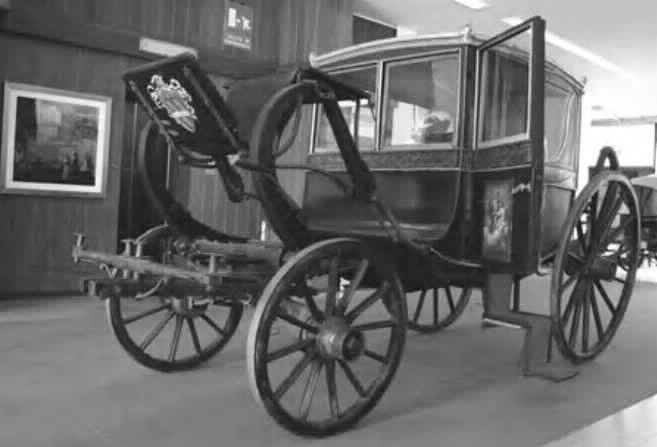
\includegraphics[width=0.4\textwidth]{2.1.png}
	\caption{This coach, built around 1650, shows a suspension made by four leaf springs and leader belts (National Automobile Museum of Torino). \cite{genta2014motorcar}
	}
	\label{fig:coach}
\end{figure}


\subsection{Suspension system evolution}
\begin{enumerate}
	\item \textbf{Passive Suspension Systems (Before 1980s):}
	\begin{itemize}
		\item Early automotive suspension systems were mostly passive, relying on mechanical components such as springs and dampers to absorb shocks and vibrations.
		\item These systems were simple and cost-effective but offered limited adaptability to varying road conditions.
	\end{itemize}
	\item \textbf{Active Suspension Systems (1980s - 1990s):}
	\begin{itemize}
		
		\item The concept of active suspension, which actively adjusts the suspension settings in response to changing road conditions, gained popularity in the 1980s.
		\item One of the pioneering examples was the development of the Lotus Active Suspension in Formula 1 in the late 1980s.
		\item Some high-end road cars began to incorporate active suspension systems in the late 1980s and early 1990s, including models from manufacturers like Citroën and Cadillac.
		\item Active suspension systems used sensors to monitor various factors, and electronic control systems adjusted the suspension settings in real-time to optimize ride comfort and handling.
	\end{itemize}
	
	\item \textbf{Semi-Active Suspension Systems (1990s - Present):}
	\begin{itemize}
		
		\item Semi-active suspension systems represent a middle ground between passive and active systems.
		\item In a semi-active system, the suspension settings are adjusted in real-time, but they typically do not provide as much active control as fully active systems.
		\item Popular semi-active systems include electronically controlled shock absorbers (e.g., Delphi's MagneRide) that can adjust damping rates based on driving conditions.
		\item These systems offer improved ride quality and handling without the complexity and cost associated with fully active systems.
	\end{itemize}
	
	\item \textbf{Recent Developments (2000s - Present):}
	\begin{itemize}
		
		\item Advancements in sensor technology, computing power, and materials have allowed for more sophisticated suspension systems.
		\item Active and semi-active suspension systems continue to evolve, with a focus on enhancing performance, safety, and comfort.
		\item Some modern high-performance and luxury vehicles feature advanced adaptive suspension systems that can adjust multiple parameters, including ride height, stiffness, and damping rates.
	\end{itemize}
\end{enumerate}
The semi-, figure \ref{fig:semi and active} (a), and fully-, figure \ref{fig:semi and active} (b), active suspension system are introduced. \cite{alashtari2023fuzzy}

\begin{figure}[H]
	\centering
	\begin{subfigure}{.35\textwidth}
		\centering
		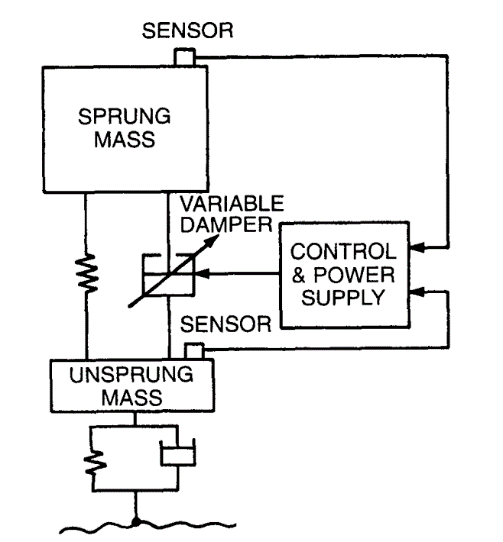
\includegraphics[width=\textwidth]{semi.png}
		\subcaption*{(a)}
	\end{subfigure}%
	\begin{subfigure}{.35\textwidth}
		\centering
		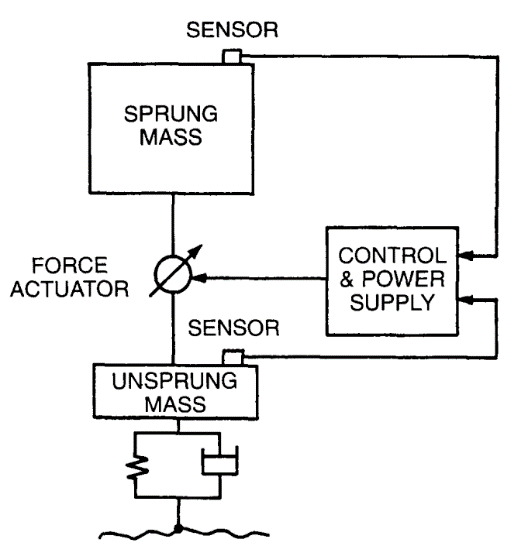
\includegraphics[width=\textwidth]{active.png}
		\subcaption*{(b)}
	\end{subfigure}
	\caption{Schematics of (a) Semi-active and (b) Fully-active suspension systems \cite{wong2001theory}}
	\label{fig:semi and active}
\end{figure}

Active suspension system is even beneficial for the HVG (Heavy Goods Vehicle) in case of the vehicle negotiating a turn.

\begin{figure}[H]
	\centering
	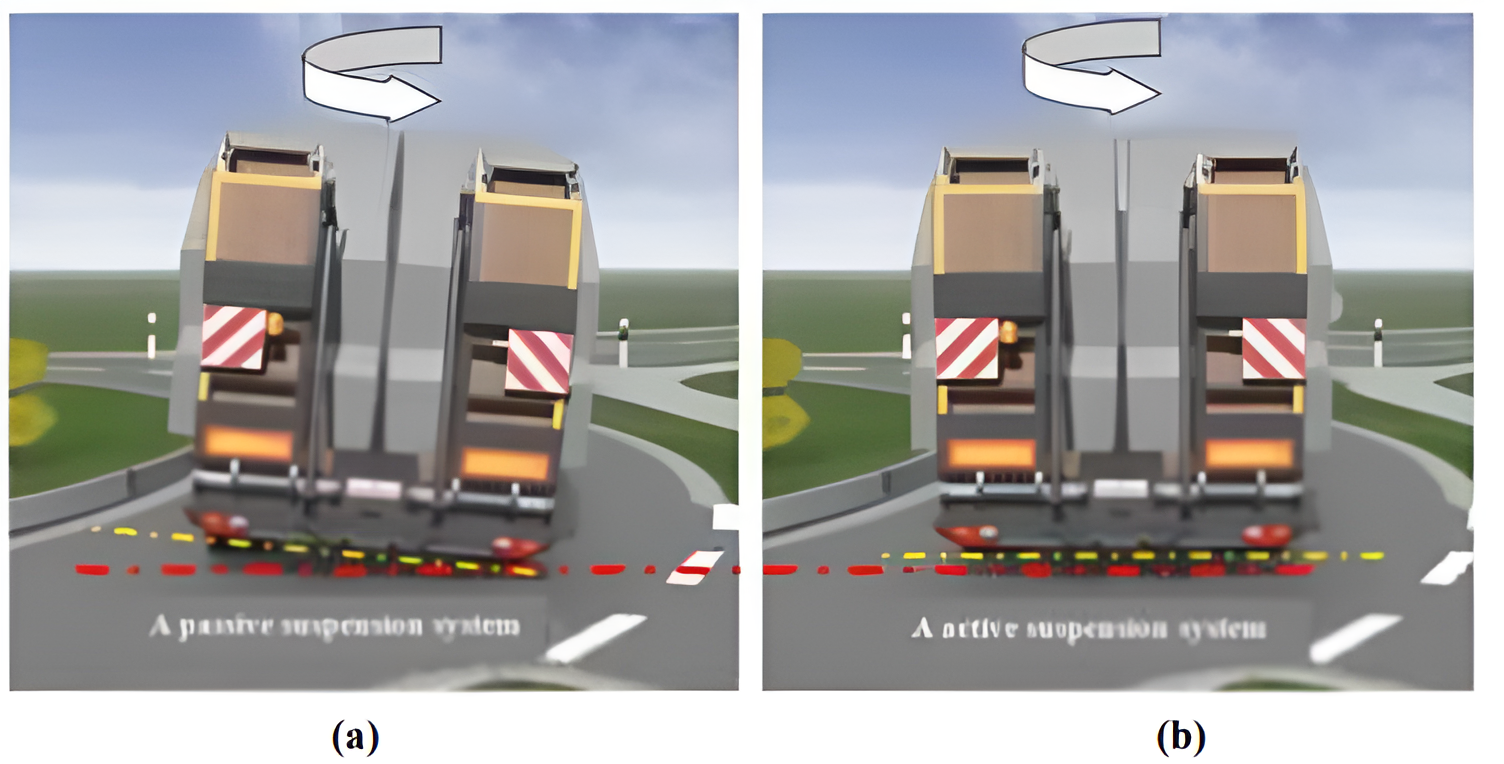
\includegraphics[width=.4\linewidth]{rolldef.png}
	\caption{Difference between the behavior of the truck body in a curve: with passive suspension (a) and with active suspension (b). \cite{hamza2022intelligent}}
	\label{fig:rolldef}
\end{figure}

\section{Recent Research}
\subsection{PID controller}
Many studies have explored various control strategies for active suspension systems over the last few decades. One of the commonly used approaches is the PID (Proportional-Integral-Derivative) algorithm, which was employed by \cite{duong2022modeling} to control the dynamics of active suspension systems. The PID controller operates in three distinct stages, each corresponding to one of the three tuning coefficients: $K_p$ (proportional), $K_D$ (derivative), and $K_i$ (integral). These coefficients can either be self-tuned through adaptive techniques or selected using standard methods like Ziegler-Nichols’s method, which is a heuristic approach to tuning PID controllers based on system response characteristics \cite{huba2021making}. This method helps achieve a balance between the system's stability and response speed.

However, the effectiveness of PID controllers often suffers from limitations in complex or nonlinear systems, where manual tuning or standard methods may not yield optimal results. To address these challenges, alternative approaches have been explored. For instance, \cite{chen2018modelling} applied the Fuzzy logic algorithm to tune the PID controller’s variables dynamically based on real-time excitation signals from the road. Fuzzy logic controllers can handle imprecision and uncertainty, offering a more adaptable solution in environments with unpredictable disturbances. Another advanced approach involves using Genetic Algorithms (GA) to optimize the PID controller’s parameters. The GA, based on principles of natural selection and genetics, can search for optimal parameter values by evaluating fitness over successive generations. This technique was demonstrated by \cite{metered2018optimized}, who applied it to fine-tune the PID controller. The GA solution allows for more flexibility in choosing optimal values for $K_p$, $K_D$, and $K_i$, adjusting to varying system conditions. The size of the population and the number of generations required for convergence are typically determined by the designer’s experience and the complexity of the system.

In contrast to the GA, the Particle Swarm Optimization (PSO) method offers another optimization technique inspired by the social behaviors of animals. PSO mimics the flocking behavior of birds or the schooling behavior of fish, where individual particles (agents) adjust their positions based on their own experience and the collective experience of their neighbors. This swarm-based approach was used by \cite{al2015quarter} to optimize the PID controller’s coefficients. The PSO algorithm is particularly useful for problems with a large number of variables and complex search spaces, as it can efficiently explore the solution space without requiring detailed knowledge of the system’s underlying dynamics.

Moreover, numerous other intelligent algorithms, such as Ant Colony Optimization (ACO) and Bee Colony Optimization (BCO), have also been explored for the optimal search of controller parameters. These bio-inspired algorithms exhibit strong performance in dynamic optimization problems, as they can adjust to system changes over time \cite{dahunsi2020proportional+}. These algorithms, like PSO and GA, offer robust alternatives to traditional optimization techniques by incorporating flexibility and adaptability.

However, when dealing with complex systems involving multiple controlled objects, a single PID controller might not be sufficient to handle all the required parameters simultaneously. In such cases, one solution is to use multiple PID controllers, each responsible for controlling different aspects or subsystems of the overall system. \cite{nguyen2021improving} explored this approach, where multiple PID controllers were used in parallel to handle the multiple degrees of freedom in an active suspension system. This method can improve performance by distributing the control efforts across different subsystems, thus ensuring better overall system behavior.

\subsection{LQR controller}
The Linear-Quadratic Regulator (LQR) controller is increasingly used to replace conventional Proportional-Integral-Derivative (PID) controllers, particularly in Multi-Input Multi-Output (MIMO) systems where multiple variables need to be controlled simultaneously \cite{wu2021multi}. The key advantage of the LQR controller lies in its ability to optimize the system’s performance by minimizing a predefined cost function, thereby improving the stability and efficiency of the system \cite{rodriguez2021active}. The optimization process involves minimizing a cost function that balances both state variables and control inputs, ensuring the system's behavior is optimal. To implement the LQR controller, the system’s mathematical model must be represented in state-space form, where the system dynamics are captured by a set of linear differential equations expressed as a state matrix \cite{nguyen2022application}. This allows for the precise calculation of the control input that minimizes the cost function at any given time.

A significant extension of the LQR controller is the Linear-Quadratic-Gaussian (LQG) controller, which combines the LQR framework with a Gaussian filter. The LQG controller incorporates the ability to estimate system states in the presence of noise and uncertainty, making it more robust in real-world applications. By combining state estimation techniques, such as Kalman filtering, with LQR control, the LQG controller can address uncertainties in system modeling and measurement, providing better control performance in dynamic environments \cite{xia2015linear}.

Recent advancements in Linear Quadratic Regulator (LQR) control have contributed significantly to the evolution of control theory, leading to improvements in both stability and applicability. One of the notable developments is the revisitation of the LQR problem for singular systems. Researchers have focused on extending the traditional LQR techniques to handle singular systems, where the system dynamics are not fully controllable or observable in the standard sense. These singular LQR techniques help broaden the applicability of LQR controllers to more complex and unconventional systems \cite{lqr_singular_systems}.

Furthermore, the role of predictions in enhancing LQR performance has been explored, especially in online control scenarios under stochastic and adversarial disturbances. By incorporating predictive models, LQR controllers can anticipate future system states and adjust the control actions proactively, improving the system's robustness against uncertainties and disturbances \cite{lqr_predictions}. In addition, data-driven approaches have gained traction, with researchers proposing LQR frameworks that rely on recursive learning algorithms and policy gradient methods. These data-driven LQR frameworks not only ensure stability but also allow the system to adapt to changing conditions by learning from past experiences, making them suitable for modern, adaptive control systems \cite{lqr_stability_recursive}.
	
\textbf{The above methods are only used for linear objects. If the object is nonlinear, more complex algorithms need to be used such as SMC MPC and RL.}




\subsection{SMC controller}
The Sliding Mode Control (SMC) algorithm is widely used for controlling complex nonlinear systems due to its robustness and ability to handle uncertainties and disturbances effectively \cite{meetei2021enhanced}. Kazemian et al. applied the SMC algorithm to control hydraulic actuators, which are commonly used in active suspension systems for their ability to provide precise force control. However, to simplify the modeling of the hydraulic actuator and make the control design more tractable, a linearization process is often performed. This process, which helps approximate the nonlinearities of the actuator, was outlined by Nguyen \cite{nguyen2021advance}. By linearizing the system, it becomes easier to apply traditional control techniques, though it still retains the essential dynamics for practical use. Subsequently, a quarter-dynamic model that considers the influence of the actuator on the vehicle's suspension system is introduced. This model typically involves five state variables, which represent the system's key dynamic parameters, such as displacement, velocity, and force \cite{nguyen2022novel}.

According to Zhao et al. \cite{zhao2023sliding}, the sliding surface plays a crucial role in the effectiveness of the SMC algorithm. The sliding surface is a boundary that separates desirable system states from undesirable ones. In the context of active suspension systems, this surface is used to drive the system’s state to a steady condition, ensuring that the vehicle’s suspension behaves in a stable manner. Once the system reaches the sliding surface, it can travel along this surface to achieve equilibrium, effectively nullifying the impact of disturbances and uncertainties.

A common issue with SMC, however, is the phenomenon known as "chattering." Chattering occurs when the control signal oscillates at high frequencies with small amplitudes, which can lead to undesirable vibrations in the system and potentially cause wear and tear on mechanical components. This issue is particularly problematic in applications like active suspension systems, where smooth control is essential for ride comfort. To mitigate chattering, researchers have proposed combining the SMC algorithm with other control strategies, such as Proportional-Integral-Derivative (PID) controllers or Fuzzy Logic controllers. For instance, Hsiao and Wang \cite{hsiao2022evaluation} introduced an innovative algorithm that integrates SMC with Fuzzy Logic, resulting in a Self-tuning Fuzzy Sliding Mode Controller (STFSMC). The fuzzy logic component allows for adaptive tuning of the control parameters, which helps reduce chattering while maintaining the robustness of the SMC algorithm.

Another approach, suggested by Suhail et al. \cite{suhail2022adaptive}, is the use of the Adaptive Sliding Mode Control (ASMC) algorithm. This method adapts the sliding mode controller in real-time, adjusting its parameters based on the system’s changing conditions. By doing so, it enhances the controller's performance and minimizes the chattering phenomenon. The combination of adaptive control and SMC offers an effective solution to the challenges of controlling nonlinear active suspension systems. Studies have shown that using such advanced control methods significantly improves ride comfort by optimizing the suspension's response to road disturbances \cite{wang2018nonlinear}. Furthermore, numerous other advanced control strategies have been applied to active suspension systems, each bringing high levels of efficiency, adaptability, and precision, making them highly suitable for modern automotive applications.
	
\subsection{RL controller}
Recent advancements in the application of reinforcement learning (RL) for active suspension systems have yielded promising results, particularly in enhancing ride comfort and vehicle stability. Reinforcement learning, with its ability to adapt and optimize in real-time, offers a dynamic approach to controlling active suspension systems. For instance, a study on deep reinforcement learning for active suspension control demonstrates its potential to meet the stringent ISO 2631-5 comfort requirements, which assess human exposure to vibration during vehicle operation \cite{deep_rl_suspension}. This study showcases how deep RL algorithms can effectively minimize vibrations and improve comfort by learning to adjust suspension parameters to various road conditions. Another research effort introduced a TD3-based control algorithm, specifically designed to address actuator delays in active suspension systems. The TD3 algorithm, known for its stability and efficiency in continuous action spaces, proves to be particularly useful in reducing the negative impact of actuator delays on system performance, resulting in better responsiveness and smoother ride quality \cite{td3_active_suspension}.

The optimization of full-vehicle active suspension systems using advanced reinforcement learning controllers has also been extensively explored, leading to significant improvements in both ride comfort and vehicle dynamics. Full-vehicle suspension systems are often subjected to a variety of road irregularities, vehicle loads, and driving conditions, making their control more complex. However, RL controllers, which can learn from these real-world variations, have shown considerable success in optimizing suspension behavior. These controllers can continuously adapt to changing conditions, leading to more efficient suspension responses and improved overall ride comfort \cite{ai_rl_full_vehicle}. Similarly, RL-based vibration control for half-car active suspension systems has demonstrated the effectiveness of adaptive dynamic programming (ADP) algorithms in reducing road-induced vibrations and improving the damping characteristics of the system. These algorithms learn to dynamically adjust control parameters, which helps to suppress unwanted vibrations that affect vehicle stability and passenger comfort \cite{rl_half_car}.

The sim-to-real transfer of active suspension control has become an essential area of research, with the goal of bridging the gap between simulated environments and real-world applications. RL-based models are often trained in idealized simulations, but transferring these models to real-world systems can present significant challenges due to model discrepancies, noise, and environmental variations. To address this, researchers have developed methods that help RL controllers generalize well from simulation to real-world deployment, ensuring they can adapt to the unpredictable nature of real-world driving conditions. This process is crucial for making RL-based active suspension systems viable in commercial vehicles \cite{sim_to_real_rl}. Additionally, a novel approach using a closed-chain five-bar active suspension system integrated with deep reinforcement learning has shown promising results in both vehicle stability and obstacle traversal. This closed-chain configuration, which involves complex mechanical linkages, benefits from RL’s ability to optimize suspension control in real-time, particularly when navigating rough or uneven terrain \cite{closed_chain_rl}.

Research into magnetorheological (MR)-damped vehicle suspension systems has also been explored using RL techniques. MR dampers, which offer the ability to adjust damping properties in response to changing driving conditions, are well-suited for use in active suspension systems. RL has proven to be highly effective in fine-tuning these dampers for optimal performance. In particular, studies have shown that the TD3 algorithm significantly outperforms traditional control strategies, particularly in terms of system adaptability and robustness. By learning from experience, the RL-based controller can adjust the damping in real time, providing superior ride comfort and handling stability \cite{mr_damped_rl}. Finally, iterative learning-based reinforcement methods for road profile estimation and active suspension control in connected vehicles highlight the potential of collaborative frameworks in improving system performance. In connected vehicle environments, data from multiple vehicles can be shared to create more accurate road profile estimations, enabling the suspension system to anticipate road conditions ahead of time. This collaborative approach allows for more precise adjustments to suspension settings, thereby enhancing both ride comfort and vehicle stability across different driving scenarios \cite{iterative_learning_rl}.


	

%\chapter{Physical Model}
%This chapter outlines the methodology employed to achieve the project objective. Firstly, a suitable quarter-car model for the active suspension system is selected. Subsequently, a mathematical model is derived, followed by its representation in state-space form. Controllability analysis is then performed on the system. Based on these findings, the following chapter delves into the implementation and evaluation of various control strategies designed to enhance the performance of the active suspension system.

\section{Two-DOF Quarter Car Model}
To analyze the parameters related to the suspension system, a simplified quarter-car model, as shown in \ref{fig:m1}(a), was utilized. The quarter-car model was chosen due to its simplicity and common use in analyzing the vertical vibrations caused by railway disturbances in vehicle dynamic models.

The vehicle's mass is divided into two: the sprung mass (representing the vehicle body) and the unsprung mass (tire). Suspension springs and dampers connect the sprung and unsprung masses and the road.

Both the transverse and longitudinal deflections are considered insignificant compared to the vertical deflections of the suspension system. For the passive suspension system is shown in \ref{fig:m1}(b).

\begin{figure}[H]
	\centering
	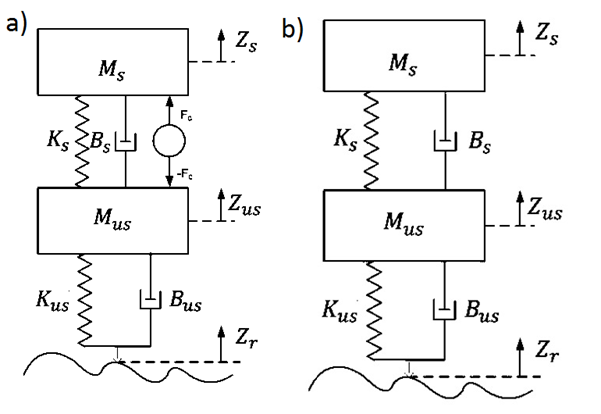
\includegraphics[width=0.4\linewidth]{model1.png}
	\caption{Active suspension system (a) and Passive suspension (b).}
	\label{fig:m1}\cite{lqr_acti}
\end{figure}

\begin{table}[H]
	\centering
	\caption{Parameters of Quarter Car Model.}
	\begin{tabular}{l|l}
		\hline
		$M_s$ & Vehicle body mass or sprung mass. \\
		$M_{us}$ & Unsprung mass (Tire, wheel, brake caliper, suspension links, etc.) \\
		$K_s$ & Spring constant for the sprung mass. \\
		$K_{us}$ & Spring constant for the unsprung mass. \\
		$B_s$ & Inherent damping coefficient for the suspension system. \\
		$B_{us}$ & Inherent damping coefficient for vehicle wheel assembly. \\
		$F_c$ & The active suspensions actuator control force. \\
		$Z_s$ & Vehicle (sprung mass) body displacement. \\
		$Z_{us}$ & Vehicles wheel displacement and the unsprung masses displacement \\
		$Z_r$ & Excitation due to the railway disturbance. \\
		\hline
	\end{tabular}
	\label{table:qcm_image}
\end{table}

\newpage
\subsection{Passive Suspension Model}
The parameters for the PSS are given in the following table:

\begin{table}[h]
	\centering
	\caption{Passive Model Parameters}
	\begin{tabular}{lccc}
		
		\hline
		\textbf{Parameter} & \textbf{Symbol} & \textbf{Value}  & \textbf{Unit}  \\
		\hline
		
		Sprung mass & \( M\)& 30 & kg\\
		Unsprung mass & \( m \)& 13 & kg\\
		Spring stiffness & \( k \)& 6921 & N/m\\ 
		Tire stiffness & \( k_{t} \)& 81000 & N/m\\
		Damper average damping coefficient & \( b_{s} \)& 900 & N s/m\\
		Tire damping coefficient & \( b_{tr} \)& 0 & N s/m\\
		
		\hline
		\label{table:Parameter}
	\end{tabular}
\end{table}
\begin{figure}[H]
	\centering
	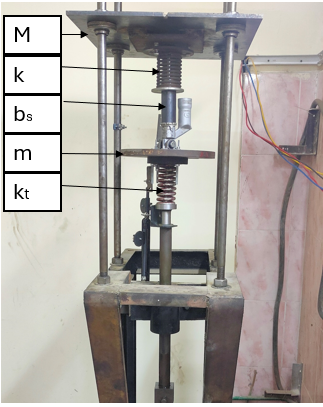
\includegraphics[width=0.45\textwidth]{layout labeled.png}
	\caption{PSS Physical Model, by Ain Shams Univresity Students as Graduation Project, Fall 2024, Automotive Department.}
	\label{fig:Passive layout}
\end{figure}

\newpage
\subsection{Active Suspension Model}
The parameters of the modified system is listed in the table below.

\begin{table}[h]
	\centering
	\caption{Active Model Parameters}
	\begin{tabular}{lccc}
		
		\hline
		\textbf{Parameter} & \textbf{Symbol} & \textbf{Value}  & \textbf{Unit}  \\
		\hline
		
		Sprung mass & \( M \)& 34 & kg\\
		Unsprung mass & \( m \)& 11 & kg\\
		Spring stiffness & \( k \)& 6921 & N/m\\ 
		Tire stiffness & \( k_{t} \)& 81000 & N/m\\
		\hline
		\label{table:Parameter}
	\end{tabular}
\end{table}

The setup of the modified Active suspension System is shown in the following figure:

\begin{figure}[H]
	\centering
	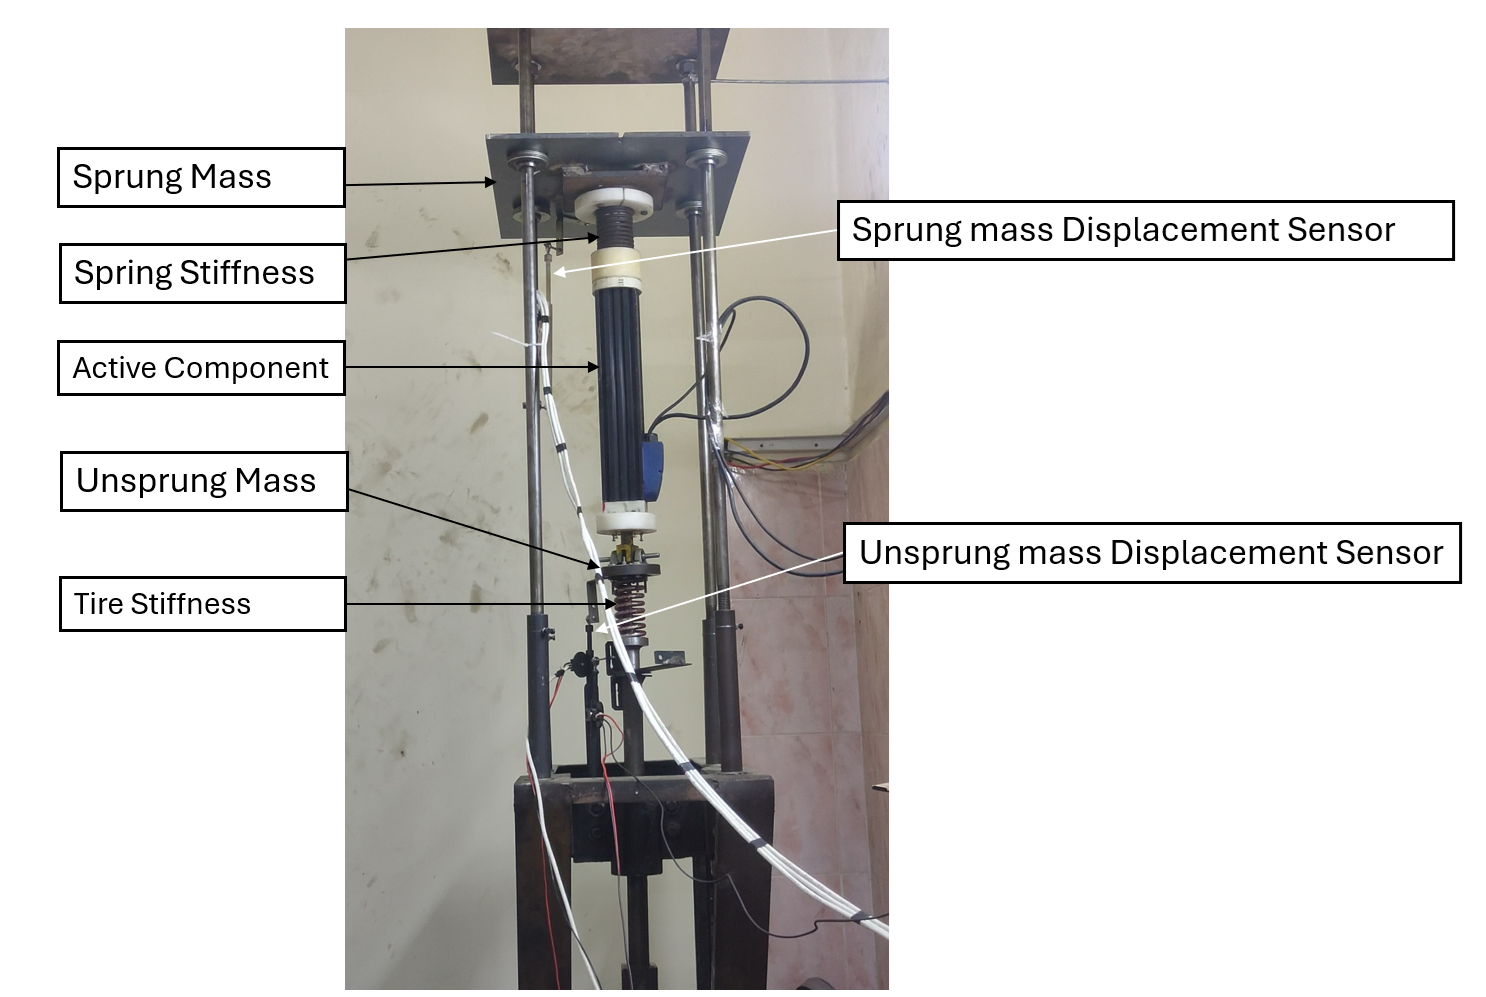
\includegraphics[width=0.9\textwidth]{Active Setup.png}
	\caption{ASS Physical Model, by Ain Shams Univresity Students as Graduation Project, Spring 2024, Automotive Department.}
	\label{fig:Active schematic diagram}	
\end{figure}


\newpage
\subsection{Equation Of Motion}

\textbf{Sprung Mass}
\begin{equation}
M_s\ddot{Z}_s = B_s\dot{Z}_{us} - B_s\dot{Z}_s - K_s(Z_s - Z_{us}) + F_c
\end{equation}

\begin{equation}
\ddot{Z}_s = \frac{B_s\dot{Z}_{us}}{M_s} - \frac{B_s\dot{Z}_s}{M_s} - \frac{K_s(Z_s - Z_{us})}{M_s} + \frac{1}{M_s}F_c
\end{equation}

\textbf{Unsprung Mass}
\begin{equation}
M_{us}\ddot{Z}_{us} = -B_s\dot{Z}_{us} - B_{us}\dot{Z}_{us} + B_s\dot{Z}_s + B_{us}\dot{Z}_r - K_s(Z_{us} - Z_s) - K_{us}(Z_{us} - Z_r) - F_c
\end{equation}\\


\begin{equation}
\ddot{Z}_{us} = -\frac{B_s\dot{Z}_{us}}{M_{us}} - \frac{B_{us}\dot{Z}_{us}}{M_{us}} + \frac{B_s\dot{Z}_s}{M_{us}} + \frac{B_{us}\dot{Z}_r}{M_{us}} - \frac{K_s(Z_{us} - Z_s)}{M_{us}} - \frac{K_{us}(Z_{us} - Z_r)}{M_{us}} - \frac{1}{M_{us}}F_c
\end{equation}\\

\subsection{State Space Model}
A state-space representation is a mathematical model used in modern control theory and system analysis to describe the behavior of a dynamic system. It offers a concise and systematic approach to representing the evolution of a system over time. In contrast to the frequency-domain representation (e.g., transfer functions), which characterizes a system's input-output relationship in terms of frequencies, the state-space representation provides a time-domain description.\\

\textbf{The general state-space representation is given by the following:}
$$\dot{x}_{(t)}=Ax_{(t)}+Bu_{(t)}$$
$$y_{(t)}=Cx_{(t)}+Du_{(t)}$$

\begin{itemize}
	\item $x$: State variables vector.
	\item $\dot{x}$: Represents the time derivative of the state variables vector.
	\item $y$: Output vector.
	\item $u$: Input vector.
	\item $A$: System matrix.
	\item $B$: Input matrix.
	\item $C$: Output matrix.
	\item $D$: Feedforward matrix.\\
\end{itemize}


\begin{table}[h!] % You can adjust the placement options (h!, t, b, p)
	\centering
	\caption{State Variables} 
	\begin{tabular}{|c|c|}
		\hline
		\textbf{Variable} & \textbf{Description} \\ \hline
		$X_1 = Z_s - Z_{us}$ & suspension travel \\ \hline
		$X_2 = \dot{Z}_s$ & sprung mass velocity \\ \hline
		$X_3 = Z_{us} - Z_r$ & wheel deflection \\ \hline
		$X_4 = \dot{Z}_{us}$ & wheel vertical velocity \\ \hline
	\end{tabular}
\end{table}



\newpage
\textbf{Inputs:} We will consider the input $\boldsymbol{u}$ into the system as the road disturbance velocity $\dot{Z}_r$ and the actuator input $F_c$.\\

\textbf{Outputs:} We will consider outputs $\boldsymbol{y}$ from the system as the suspension travel $Z_s-Z_{us}$ and the vehicle body (sprung mass) acceleration $\ddot{Z}_s$.\\

Using the above equations of motion, the state-space model of the active suspension system can easily be obtained and be written in the matrix form shown below:

\begin{equation}
\begin{bmatrix}
	\dot{x}_1 \\
	\dot{x}_2 \\
	\dot{x}_3 \\
	\dot{x}_4
\end{bmatrix} = 
\begin{bmatrix}
	0 & 1 & 0 & -1 \\
	-\frac{K_s}{M_s} & -\frac{B_s}{M_s} & 0 & \frac{B_s}{M_s} \\
	0 & 0 & 0 & 1 \\
	\frac{K_s}{M_{us}} & \frac{B_s}{M_{us}} & -\frac{K_{us}}{M_{us}} & -\frac{B_s + B_{us}}{M_{us}} 
\end{bmatrix}
\begin{bmatrix}
	x_1 \\
	x_2 \\
	x_3 \\
	x_4
\end{bmatrix} + 
\begin{bmatrix}
	0 & 0 \\
	0 & \frac{1}{M_{s}} \\
	-1 & 0 \\
	\frac{B_{us}}{M_{us}} & -\frac{1}{M_{us}} \\
\end{bmatrix}
\begin{bmatrix}
	\dot{Z}_r \\
	F_c
\end{bmatrix}
\end{equation}


\begin{equation}
\begin{bmatrix}
	Y_1 \\
	Y_2
\end{bmatrix} = 
\begin{bmatrix}
	1 & 0 & 0 & 0 \\
	-\frac{K_s}{M_s} & -\frac{B_s}{M_s} & 0 & \frac{B_s}{M_s} 
\end{bmatrix}
\begin{bmatrix}
	X_1 \\
	X_2 \\
	X_3 \\
	X_4
\end{bmatrix} + 
\begin{bmatrix}
	0 & 0 \\
	0 & \frac{1}{M_s}
\end{bmatrix}
\begin{bmatrix}
	\dot{Z}_r \\
	F_c
\end{bmatrix}
\end{equation}







\section{State Space Controllability}
State-space controllability refers to the ability to drive a system from any initial state to any desired state within a finite time using an appropriate control input. A linear time-invariant (LTI) system represented in state-space form, is controllable if the controllability matrix has full rank. When this condition is met, it ensures that the system's states can be influenced by the control input, enabling effective feedback control design.\newline

$\mathcal{C} = \left[ \begin{matrix}
	B & AB & A^2B & \cdots & A^{n-1}B
\end{matrix} \right]$\newline

$rank(\mathcal{C}) = n$


\begin{verbatim}
	% MATLAB script
	ms  = 34;           % Sprung Mass (kg)
	mus = 11;           % Unsprung Mass (kg)
	ks  = 6921;         % Suspension Stiffness (N/m)
	kus = 81000;        % Wheel stiffness (N/m)
	bs  = 0;            % Suspension Inherent Damping coefficient (sec/m)
	bus = 0;            % Wheel Inhenrent Damping coefficient (sec/m)
	
	%% System Dynamics for the Active Suspension system.
	A = [ 0 1 0 -1 ;
	-ks/ms -bs/ms 0 bs/ms;
	0 0 0 1; 
	ks/mus bs/mus -kus/mus -(bs+bus)/mus];
	
	B = [0  0 ; 
	0 1/ms ; 
	-1  0 ;
	bus/mus -1/mus ];
	
	C = [ 1 0 0 0 ; 
	-ks/ms -bs/ms 0 bs/ms ];
	
	D = [0 0;
	0 0;
	0 0;
	0 0;
	0 0;
	0 1/ms];
	
	%% Controllability
	rank(ctrb(A,B))
\end{verbatim}

The following figure shows that the system is controllable, because its controllability matrix is full rank which is equal to the number of states.\newline

\begin{figure}[H]
	\centering
	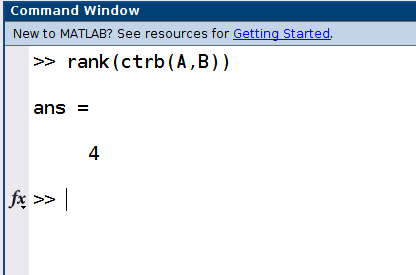
\includegraphics[width=0.4\textwidth]{ctrb.png}
	\caption{Conrollability matrix is full rank}
	\label{fig:ctrb}	
\end{figure}


\section{Road Disturbance Profile}
The slider-crank mechanism as shown in\ref{fig:sliderr} is used to simulate road. This mechanism converts the rotational motion of a crank into the linear motion of a slider, effectively replicating the vertical displacement experienced by a vehicle's suspension system when driving over uneven road surfaces which can change road amplitude by changing eccentricity from crank disk.
\begin{figure}[H]
	\centering
	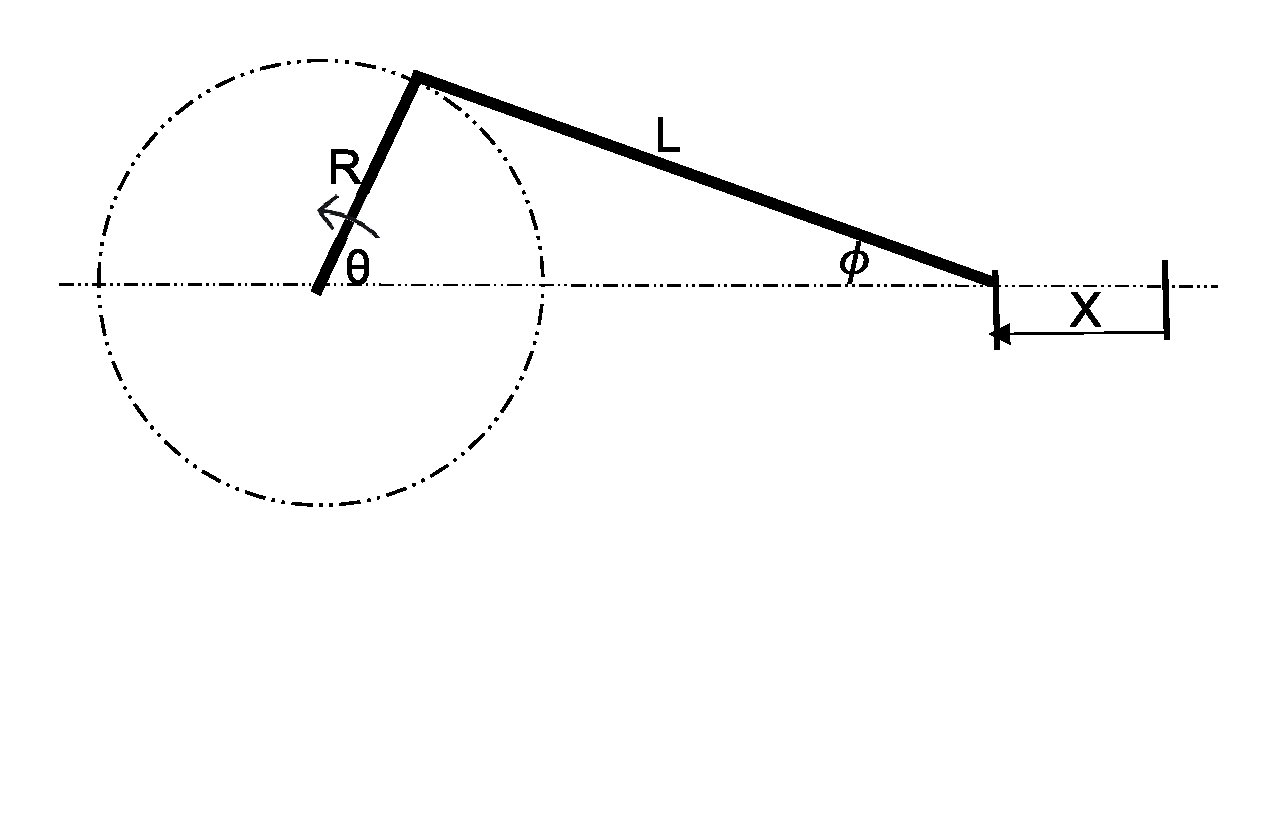
\includegraphics[trim=0cm 4cm 0cm 0cm, clip, width=1\linewidth]{sliderr.pdf}
	\caption{the slider crank mechanism}
	\label{fig:sliderr}
\end{figure}

\begin{itemize}
	\item $R$: Length of the crank
	\item $L$: Length of the connecting rod
	\item $\theta $: Angle of the crank 
	\item $x$: Position of the slider
\end{itemize}
\newpage
\subsection*{Kinematic Equations}

The position \( x \) of the slider can be determined using the crank angle \( \theta \) and \( \phi \) be the angle of the connecting rod with the horizontal. The position \( x \) of the slider can be expressed as:


\begin{equation}
	x = R \left[ 1 - \cos \theta + n - \sqrt{n^2 - \sin^2 \theta} \right] 
\end{equation}

since \( n = \frac{L}{R} \).


\chapter{Mathematical Model}
\section{Two-DOF Quarter Car Model}
To analyze the parameters related to the suspension system, a simplified quarter-car model, as shown in \ref{fig:m1}(a), was utilized. The quarter-car model was chosen due to its simplicity and common use in analyzing the vertical vibrations caused by railway disturbances in vehicle dynamic models.

The vehicle's mass is divided into two: the sprung mass (representing the vehicle body) and the unsprung mass (tire). Suspension springs and dampers connect the sprung and unsprung masses and the road.

Both the transverse and longitudinal deflections are considered insignificant compared to the vertical deflections of the suspension system. For the passive suspension system, the actuator force is not considered as there is no control element, as shown in \ref{fig:m1}(b).

\begin{figure}[H]
	\centering
	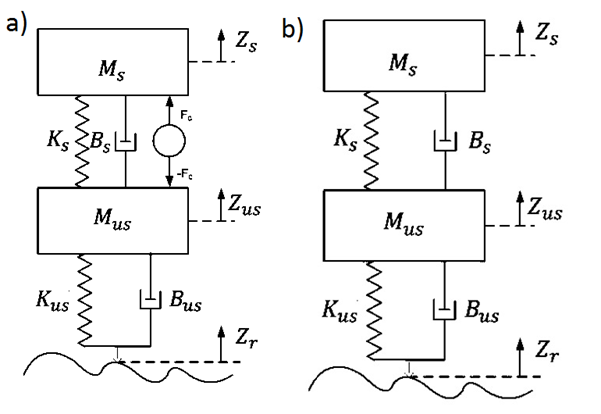
\includegraphics[width=0.4\linewidth]{model1.png}
	\caption{Active suspension system (a) and Passive suspension (b).}
	\label{fig:m1}\cite{lqr_acti}
\end{figure}

\begin{table}[H]
	\centering
	\caption{Parameters of Quarter Car Model.}
	\begin{tabular}{l|l}
		\hline
		$M_s$ & Vehicle body mass or sprung mass. \\
		$M_{us}$ & Unsprung mass (Tire, wheel, brake caliper, suspension links, etc.) \\
		$K_s$ & Spring constant for the sprung mass. \\
		$K_{us}$ & Spring constant for the unsprung mass. \\
		$B_s$ & Inherent damping coefficient for the suspension system. \\
		$B_{us}$ & Inherent damping coefficient for vehicle wheel assembly. \\
		$F_c$ & The active suspensions actuator control force. \\
		$Z_s$ & Vehicle (sprung mass) body displacement. \\
		$Z_{us}$ & Vehicles wheel displacement and the unsprung masses displacement \\
		$Z_r$ & Excitation due to the railway disturbance. \\
		\hline
	\end{tabular}
	\label{table:qcm_image}
\end{table}

\newpage
\subsection{Passive Suspension Model}
The parameters for the PSS are given in the following table:

\begin{table}[h]
	\centering
	\caption{Passive Model Parameters}
	\begin{tabular}{lccc}
		
		\hline
		\textbf{Parameter} & \textbf{Symbol} & \textbf{Value}  & \textbf{Unit}  \\
		\hline
		
		Sprung mass & \( M\)& 30 & kg\\
		Unsprung mass & \( m \)& 13 & kg\\
		Spring stiffness & \( k \)& 6921 & N/m\\ 
		Tire stiffness & \( k_{t} \)& 81000 & N/m\\
		Damper average damping coefficient & \( b_{s} \)& 900 & N s/m\\
		Tire damping coefficient & \( b_{tr} \)& 0 & N s/m\\
		
		\hline
		\label{table:Parameter}
	\end{tabular}
\end{table}
\begin{figure}[H]
	\centering
	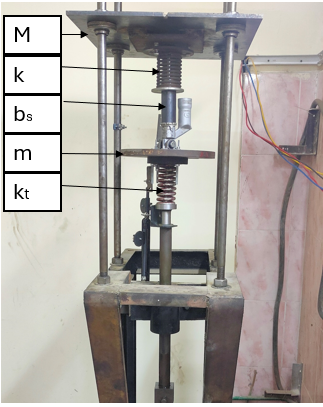
\includegraphics[width=0.45\textwidth]{layout labeled.png}
	\caption{PSS Physical Model, by Ain Shams Univresity Students as Graduation Project, Fall 2024, Automotive Department.}
	\label{fig:Passive layout}
\end{figure}

\newpage
\subsection{Active Suspension Model}
The parameters of the modified system is listed in the table below.

\begin{table}[h]
	\centering
	\caption{Active Model Parameters}
	\begin{tabular}{lccc}
		
		\hline
		\textbf{Parameter} & \textbf{Symbol} & \textbf{Value}  & \textbf{Unit}  \\
		\hline
		
		Sprung mass & \( M \)& 34 & kg\\
		Unsprung mass & \( m \)& 11 & kg\\
		Spring stiffness & \( k \)& 6921 & N/m\\ 
		Tire stiffness & \( k_{t} \)& 81000 & N/m\\
		\hline
		\label{table:Parameter}
	\end{tabular}
\end{table}

The setup of the modified Active suspension System is shown in the following figure:

\begin{figure}[H]
	\centering
	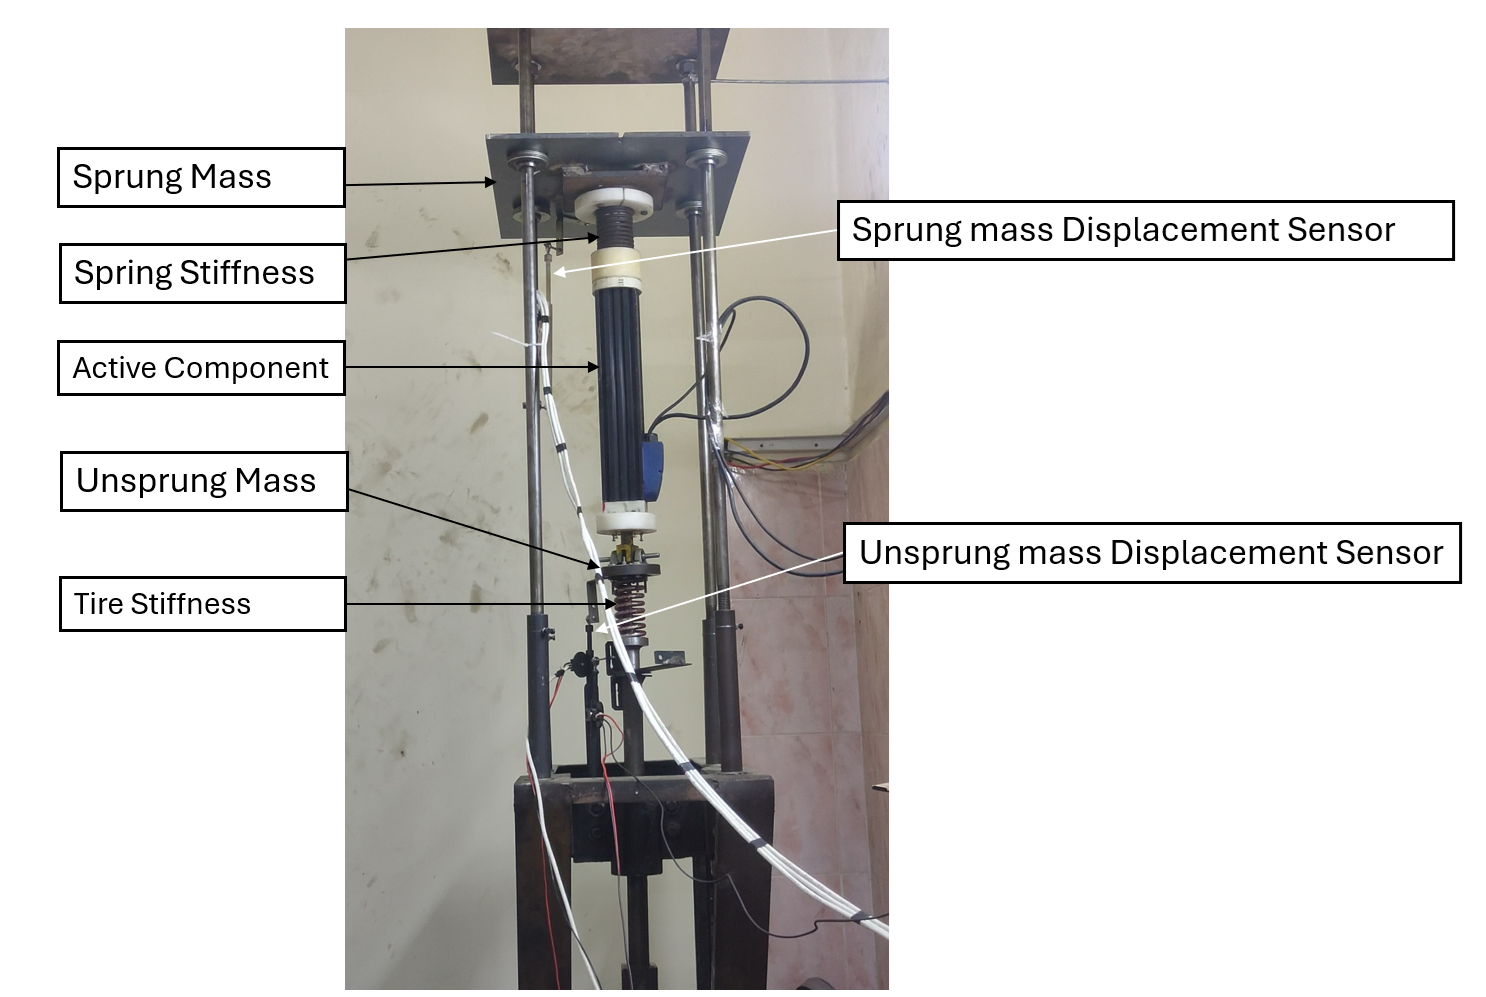
\includegraphics[width=0.9\textwidth]{Active Setup.png}
	\caption{ASS Physical Model, by Ain Shams Univresity Students as Graduation Project, Spring 2024, Automotive Department.}
	\label{fig:Active schematic diagram}	
\end{figure}


\newpage
\subsection{Equation Of Motion}

\textbf{Sprung Mass}
\begin{equation}
M_s\ddot{Z}_s = B_s\dot{Z}_{us} - B_s\dot{Z}_s - K_s(Z_s - Z_{us}) + F_c
\end{equation}

\begin{equation}
\ddot{Z}_s = \frac{B_s\dot{Z}_{us}}{M_s} - \frac{B_s\dot{Z}_s}{M_s} - \frac{K_s(Z_s - Z_{us})}{M_s} + \frac{1}{M_s}F_c
\end{equation}

\textbf{Unsprung Mass}
\begin{equation}
M_{us}\ddot{Z}_{us} = -B_s\dot{Z}_{us} - B_{us}\dot{Z}_{us} + B_s\dot{Z}_s + B_{us}\dot{Z}_r - K_s(Z_{us} - Z_s) - K_{us}(Z_{us} - Z_r) - F_c
\end{equation}\\


\begin{equation}
\ddot{Z}_{us} = -\frac{B_s\dot{Z}_{us}}{M_{us}} - \frac{B_{us}\dot{Z}_{us}}{M_{us}} + \frac{B_s\dot{Z}_s}{M_{us}} + \frac{B_{us}\dot{Z}_r}{M_{us}} - \frac{K_s(Z_{us} - Z_s)}{M_{us}} - \frac{K_{us}(Z_{us} - Z_r)}{M_{us}} - \frac{1}{M_{us}}F_c
\end{equation}\\

\subsection{State Space Model}
A state-space representation is a mathematical model used in modern control theory and system analysis to describe the behavior of a dynamic system. It offers a concise and systematic approach to representing the evolution of a system over time. In contrast to the frequency-domain representation (e.g., transfer functions), which characterizes a system's input-output relationship in terms of frequencies, the state-space representation provides a time-domain description.\\

\textbf{The general state-space representation is given by the following:}
$$\dot{x}_{(t)}=Ax_{(t)}+Bu_{(t)}$$
$$y_{(t)}=Cx_{(t)}+Du_{(t)}$$

\begin{itemize}
	\item $x$: State variables vector.
	\item $\dot{x}$: Represents the time derivative of the state variables vector.
	\item $y$: Output vector.
	\item $u$: Input vector.
	\item $A$: System matrix.
	\item $B$: Input matrix.
	\item $C$: Output matrix.
	\item $D$: Feedforward matrix.\\
\end{itemize}

\textbf{State variables:}
\begin{center}
	\begin{tabular}{|c|c|}
		\hline
		\textbf{Variable} & \textbf{Description} \\ \hline
		$X_1 = Z_s - Z_{us}$ & suspension travel \\ \hline
		$X_2 = \dot{Z}_s$ & sprung mass velocity \\ \hline
		$X_3 = Z_{us} - Z_r$ & wheel deflection \\ \hline
		$X_4 = \dot{Z}_{us}$ & wheel vertical velocity \\ \hline
	\end{tabular}
\end{center}

\newpage
\textbf{Inputs:} We will consider the input $\boldsymbol{u}$ into the system as the road disturbance velocity $\dot{Z}_r$ and the actuator input $F_c$.\\

\textbf{Outputs:} We will consider outputs $\boldsymbol{y}$ from the system as the suspension travel $Z_s-Z_{us}$ and the vehicle body (sprung mass) acceleration $\ddot{Z}_s$.\\

Using the above equations of motion, the state-space model of the active suspension system can easily be obtained and be written in the matrix form shown below:

\begin{equation}
\begin{bmatrix}
	\dot{x}_1 \\
	\dot{x}_2 \\
	\dot{x}_3 \\
	\dot{x}_4
\end{bmatrix} = 
\begin{bmatrix}
	0 & 1 & 0 & -1 \\
	-\frac{K_s}{M_s} & -\frac{B_s}{M_s} & 0 & \frac{B_s}{M_s} \\
	0 & 0 & 0 & 1 \\
	\frac{K_s}{M_{us}} & \frac{B_s}{M_{us}} & -\frac{K_{us}}{M_{us}} & -\frac{B_s + B_{us}}{M_{us}} 
\end{bmatrix}
\begin{bmatrix}
	x_1 \\
	x_2 \\
	x_3 \\
	x_4
\end{bmatrix} + 
\begin{bmatrix}
	0 & 0 \\
	0 & \frac{1}{M_{s}} \\
	-1 & 0 \\
	\frac{B_{us}}{M_{us}} & -\frac{1}{M_{us}} \\
\end{bmatrix}
\begin{bmatrix}
	\dot{Z}_r \\
	F_c
\end{bmatrix}
\end{equation}


\begin{equation}
\begin{bmatrix}
	Y_1 \\
	Y_2
\end{bmatrix} = 
\begin{bmatrix}
	1 & 0 & 0 & 0 \\
	-\frac{K_s}{M_s} & -\frac{B_s}{M_s} & 0 & \frac{B_s}{M_s} 
\end{bmatrix}
\begin{bmatrix}
	X_1 \\
	X_2 \\
	X_3 \\
	X_4
\end{bmatrix} + 
\begin{bmatrix}
	0 & 0 \\
	0 & \frac{1}{M_s}
\end{bmatrix}
\begin{bmatrix}
	\dot{Z}_r \\
	F_c
\end{bmatrix}
\end{equation}







\section{State Space Controllability}
State-space controllability refers to the ability to drive a system from any initial state to any desired state within a finite time using an appropriate control input. A linear time-invariant (LTI) system represented in state-space form, is controllable if the controllability matrix has full rank. When this condition is met, it ensures that the system's states can be influenced by the control input, enabling effective feedback control design.\newline

$\mathcal{C} = \left[ \begin{matrix}
	B & AB & A^2B & \cdots & A^{n-1}B
\end{matrix} \right]$\newline

$rank(\mathcal{C}) = n$


\begin{verbatim}
	% MATLAB script
	ms  = 34;           % Sprung Mass (kg)
	mus = 11;           % Unsprung Mass (kg)
	ks  = 6921;         % Suspension Stiffness (N/m)
	kus = 81000;        % Wheel stiffness (N/m)
	bs  = 0;            % Suspension Inherent Damping coefficient (sec/m)
	bus = 0;            % Wheel Inhenrent Damping coefficient (sec/m)
	
	%% System Dynamics for the Active Suspension system.
	A = [ 0 1 0 -1 ;
	-ks/ms -bs/ms 0 bs/ms;
	0 0 0 1; 
	ks/mus bs/mus -kus/mus -(bs+bus)/mus];
	
	B = [0  0 ; 
	0 1/ms ; 
	-1  0 ;
	bus/mus -1/mus ];
	
	C = [ 1 0 0 0 ; 
	-ks/ms -bs/ms 0 bs/ms ];
	
	D = [0 0;
	0 0;
	0 0;
	0 0;
	0 0;
	0 1/ms];
	
	%% Controllability
	rank(ctrb(A,B))
\end{verbatim}

The following figure shows that the system is controllable, because its controllability matrix is full rank which is equal to the number of states.\newline

\begin{figure}[H]
	\centering
	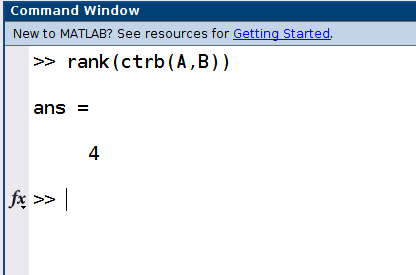
\includegraphics[width=0.4\textwidth]{ctrb.png}
	\caption{Conrollability matrix is full rank}
	\label{fig:ctrb}	
\end{figure}


\section{Road Disturbance Profile}
The slider-crank mechanism as shown in\ref{fig:sliderr} is used to simulate road. This mechanism converts the rotational motion of a crank into the linear motion of a slider, effectively replicating the vertical displacement experienced by a vehicle's suspension system when driving over uneven road surfaces which can change road amplitude by changing eccentricity from crank disk.
\begin{figure}[H]
	\centering
	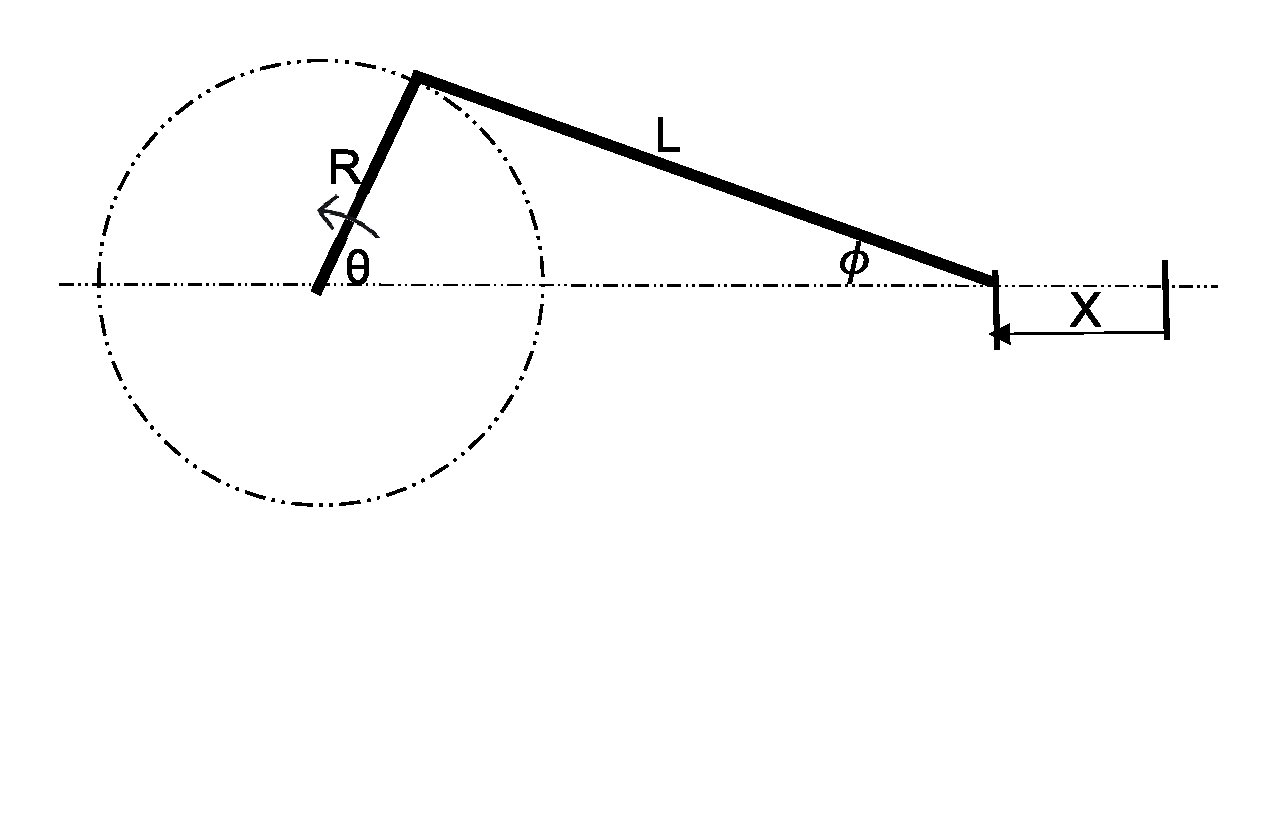
\includegraphics[trim=0cm 4cm 0cm 0cm, clip, width=1\linewidth]{sliderr.pdf}
	\caption{the slider crank mechanism}
	\label{fig:sliderr}
\end{figure}

\begin{itemize}
	\item $R$: Length of the crank
	\item $L$: Length of the connecting rod
	\item $\theta $: Angle of the crank 
	\item $x$: Position of the slider
\end{itemize}
\newpage
\subsection*{Kinematic Equations}

The position \( x \) of the slider can be determined using the crank angle \( \theta \) and \( \phi \) be the angle of the connecting rod with the horizontal. The position \( x \) of the slider can be expressed as:

\[
x = R \left[ 1 - \cos \theta + n - \sqrt{n^2 - \sin^2 \theta} \right]
\]

since \( n = \frac{L}{R} \).






%%%%%%%%%%%%%%%%%%%%%%%%%%%%%%%%%%%%%%%%%%%%%%%%%%%%%%%%%%%%%%%%%%%%%%%%%%%%

\iffalse
\section{Quarter Car Passive Suspension Model}

The vertical dynamics of the tire can be simply equated to a spring and a damping mechanism, and then the 2-DOF dynamic model as shown in figure \ref{fig:qcm} can be established.
This model is one of the most widely used suspension models, which is very important when studying vehicle dynamics, especially ride comfort and road handling characteristics. It represents the vibration behavior of the car body and the wheel. \cite{sun2020advanced}

\begin{figure}[H]
	\centering
	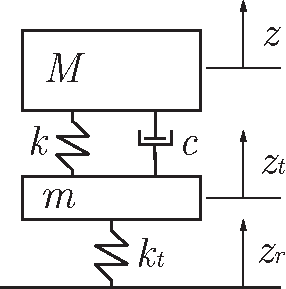
\includegraphics[width=0.4\linewidth]{qcm.pdf}
	
	\caption{Quarter Car Model\cite{researchgate_hybrid_control}.}
	\label{fig:qcm}
\end{figure}

Based on the free body diagram of the quarter car model shown in figure \ref{fig:qcm} and Newton's second law:
\begin{equation}
	m\ddot{z_t}=-k(z_t-z)-c(\dot{z_t}_-\dot{z})-k_t(z_t-z_r)
	\label{eqn:4.1}
\end{equation}
\begin{equation}
	M\ddot{z}=-k(z-z_t)-c(\dot{z}-\dot{z}_t)
	\label{eqn:4.2}
\end{equation}


\begin{table}[H]
	\centering
	\caption{Parameters of Quarter Car Model.}
	\begin{tabular}{ l|l }
		\hline
		$m$   & Unsprung mass (Tire, wheel, brake caliper, suspension links, etc.) \\
		$M$   & Quarter-car body mass                                              \\
		$k$   & Stiffness of the suspension                                        \\
		$k_t$ & Stiffness of the tire                                              \\
		$c$   & Damping coefficient of the sprung shock-absorber                   \\
		$z$   & Vertical position of the car body                                  \\
		$z_t$ & Vertical position of the unsprung mass                             \\
		$z_r$ & Vertical position of road profile                                  \\
		\hline
	\end{tabular}
	\label{table:qcm}
\end{table}


\section{Quarter Car Active Suspension Model}
With proper controlling methods, an active suspension can result in compromise
between vehicle ride comforts to road handling stableness be more improved, thus making
it an overall enhanced suspension design\cite{riduan2018review}.
Figure \ref{fig:Active schematic diagram} shows the two-degrees-of
freedom system that represents the quarter-vehicle active 
suspension model. It consists of an upper mass ($M$), 
representing the body mass (sprung mass), as well as a 
lower mass ($m$), representing the wheel mass (un-sprung 
mass), and its associated parts. The vertical motion of the 
system is described by the displacements ($z$), and($z_t$) , 
while the excitation due to road disturbance is ($z_r$). The 
suspension spring constant is ($k$), damping coefficient is 
($c$), and the tyre spring constant is ($k_t$) (the tyre damping is 
neglected). The data employed here for the quarter
vehicle system are listed in Table \ref{table:qcm}. 

Based on the free body diagram of the quarter car model shown in figure 
By applying Newton’s second law the equations of 
motion for the sprung and unsprung masses of the quarter
car suspension model are given by \cite{chiou2009using}:
\begin{figure}[H]
	\centering
	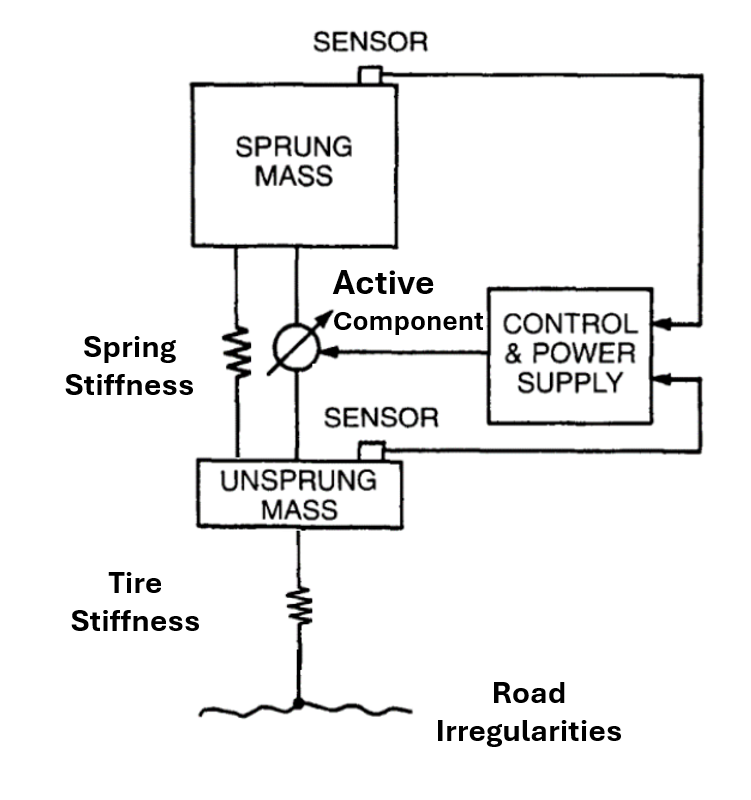
\includegraphics[width=0.4\textwidth]{Active schematic diagram.png}
	\caption{Schematic Diagram of the Modified Active Suspension System \cite{wong2001theory}}
	\label{fig:Active schematic diagram}
	
\end{figure}
\begin{equation}
	M\ddot{z} = -k(z - z_t) - F_a
	\label{eqn:4.2}
\end{equation}

\begin{equation}
	m\ddot{z_t}=-k(z_t-z)-k_t(z_t-z_r)+ F_a
	\label{eqn:4.1}
\end{equation}
\begin{table}[H]
	\centering
	\caption{Parameters of Quarter Car Model \cite{turkay2005study}}
	\begin{tabular}{ l|l }
		\hline
		$M$   & Quarter-car body mass                                              \\
		$m$   & Unsprung mass (Tire, wheel, brake caliper, suspension links, etc.) \\
		$k$   & Stiffness of the suspension                                        \\
		$k_t$ & Stiffness of the tire                                              \\
		$F_a$ &  the control force from the actuator                  \\
		$z$   & Vertical position of the car body                                  \\
		$z_t$ & Vertical position of the unsprung mass                             \\
		$z_r$ & Vertical position of road profile                                  \\
		\hline
	\end{tabular}
	\label{table:qcm}
\end{table}


In this chapter, vehicle dynamic modeling is a major step in the design of suspension systems. According to the requirement of controller design, the three dynamic models: two (DOF) quarter-car models, four DOF half-car models, and seven DOF full-car models, are used for the theoretical analysis and design of suspension systems. \cite{sun2020advanced}
We Explain Types of Road Excitation and the effect of tire radius and how these factors influence of Suspension system Model.

%%%%%%%%%%%%%%%%%%%%%%%%%%%%%%%%

\section{STATE SPACE MODEL}
A state-space representation is a mathematical model used in control theory and system analysis to describe the behavior of a dynamic system. It provides a concise and systematic way to represent the evolution of a system over time. The essential components of a state-space representation include:

\begin{itemize}
	\item State Variables (x): These are variables that describe the current state of the system. They are typically chosen to be the smallest set of variables that completely define the system at any given time.
	\item Input Variables (u): These represent the inputs or control signals applied to the system. Inputs can be manipulated to influence the system's behavior.
	\item Output Variables (y): These represent the measurable outputs of the system. Outputs are influenced by both the current state and the input signals.
	\item State Equations: These are a set of first-order differential equations that describe how the state variables evolve over time. The state equations are often expressed in matrix form as $\dot{x}=Ax+Bu$, where $x$ is the derivative of the state vector $x$, A is the state matrix, B is the input matrix, and u is the input vector.
	\item Output Equations: These equations relate the state and input variables to the output variables. They are typically expressed as $y=Cx+Du$, where $C$ is the output matrix, and $D$ is the feedforward matrix.
\end{itemize}

The state-space representation is particularly useful for analyzing and designing control systems. It allows us to apply linear algebra and matrix theory to study the system's behavior, stability, and controllability. Later, it will help us design controllers that can manipulate inputs to achieve desired system responses \cite{nguyen2023dynamic}, we will use it to represent passive quarter-car model dynamical equations (\ref{eqn:4.1}, \ref{eqn:4.2}), in this chapter we will consider only input in our system is road input $z_r$ as shown in equation \ref{eqn:ssm}, and we neglect $D$  the feedforward matrix in our model.

$$\dot{x}_{(t)}=Ax_{(t)}+Bu_{(t)}$$
$$y_{(t)}=Cx_{(t)}$$
\begin{equation}
	\centering
	\begin{bmatrix}
		\ddot{z}   \\
		\dot{z}    \\
		\ddot{z}_t \\
		\dot{z}_t  \\
	\end{bmatrix}
	=
	\begin{bmatrix}
		-c/M & -k/M & c/M  & k/M        \\
		1    & 0    & 0    & 0          \\
		c/m  & k/m  & -c/m & (-k-k_t)/m \\
		0    & 0    & 1    & 0          \\
	\end{bmatrix}
	\begin{bmatrix}
		\dot{z}   \\
		z         \\
		\dot{z}_t \\
		z_t       \\
	\end{bmatrix}
	+
	\begin{bmatrix}
		0     \\
		z  0  \\
		k_t/m \\
		0     \\
	\end{bmatrix}
	z_r
	\label{eqn:ssm}
\end{equation}
$$
y_{(t)}=
\begin{bmatrix}
	1 & 0 & 0 & 0 \\
	0 & 1 & 0 & 0 \\
	0 & 0 & 1 & 0 \\
	0 & 0 & 0 & 1 \\
	
\end{bmatrix}
\begin{bmatrix}
	\dot{z}   \\
	z         \\
	\dot{z}_t \\image
	z_t       \\
\end{bmatrix}
$$

%%%%%%%%%%%%%%%%%%%%%%%%%%%%%%%%%%%%%%%%%%%%
In this chapter we are going to validate the simulation model by comparing between the simulation results and the experimental results.
\newline
In the simulation results the road input is taken from the road input sensor to ensure the exact behavior in the real world is entered to the simulation model. So, the procedure of the validation is as follows:
\begin{itemize}
	\item Compare the road input of the Slider-Crank mechanism with the road input displacement sensor to ensure the good function of the road input excitation mechanism.
	\item Compare the unsprung mass displacement results either simulation and experimental.
	\item Compare the sprung mass displacement results either simulation and experimental.
\end{itemize}
all these results are repeated three times at different values of excitation frequencies:
\begin{itemize}
	\item 0.309 [Hz]
	\item 0.817 [Hz]
	\item 1.670 [Hz]
\end{itemize}

\section{Road Input Comparison}
\begin{itemize}
	\item 0.309 [Hz]
\end{itemize}
\begin{figure}[H]
	\centering
	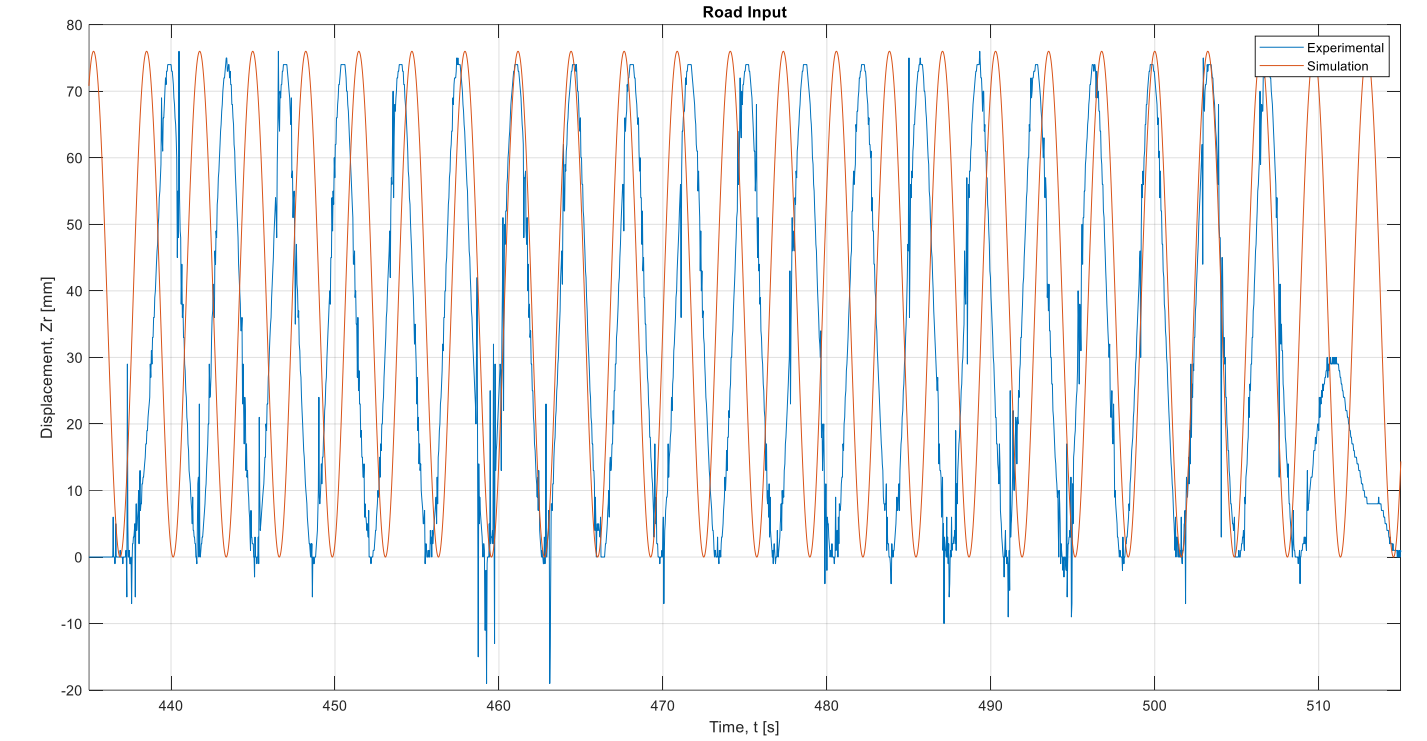
\includegraphics[width=0.9\linewidth]{figures/0.309 RI.png}
	\caption{Road Input Comparison at 0.309 [Hz]}
	\label{fig:Road Input Comparison at 0.309}
\end{figure}

\begin{itemize}
	\item 0.817 [Hz]
\end{itemize}
\begin{figure}[H]
	\centering
	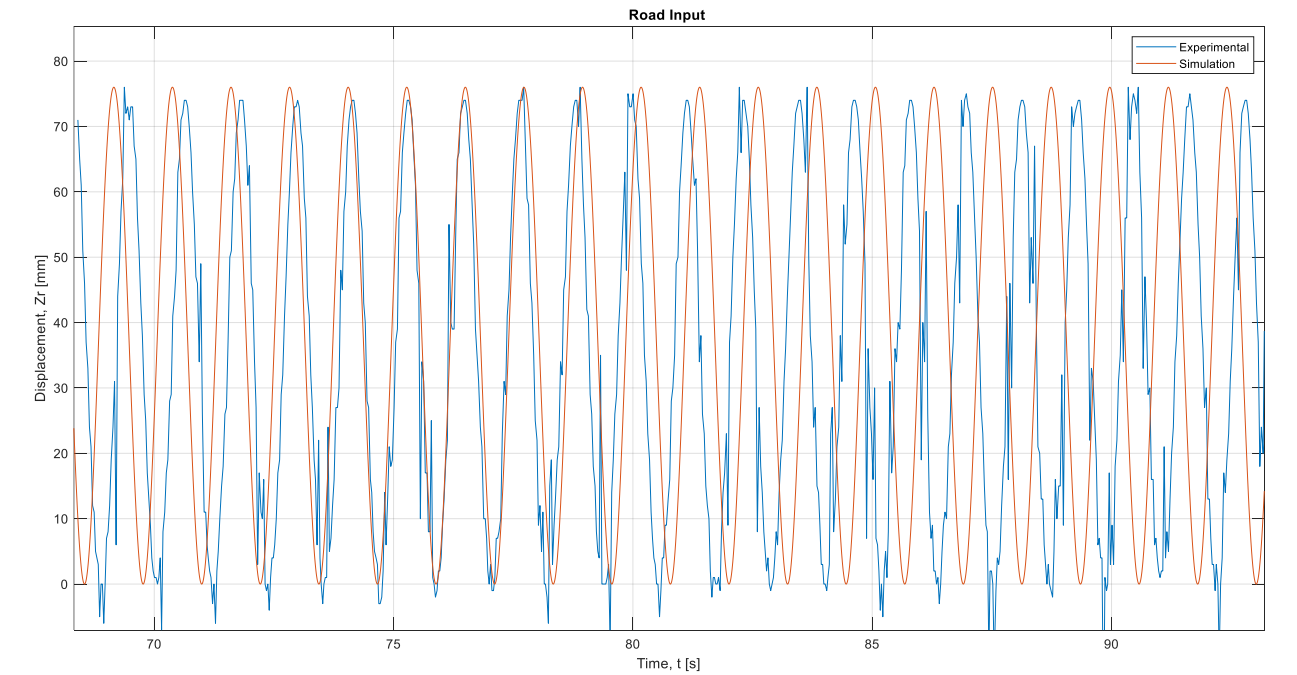
\includegraphics[width=0.99\linewidth]{figures/0.817 RI.png}
	\caption{Road Input Comparison at 0.817 [Hz]}
	\label{fig:Road Input Comparison at 0.817}
\end{figure}
\begin{itemize}
	\item 1.670 [Hz]
\end{itemize}
\begin{figure}[H]
	\centering
	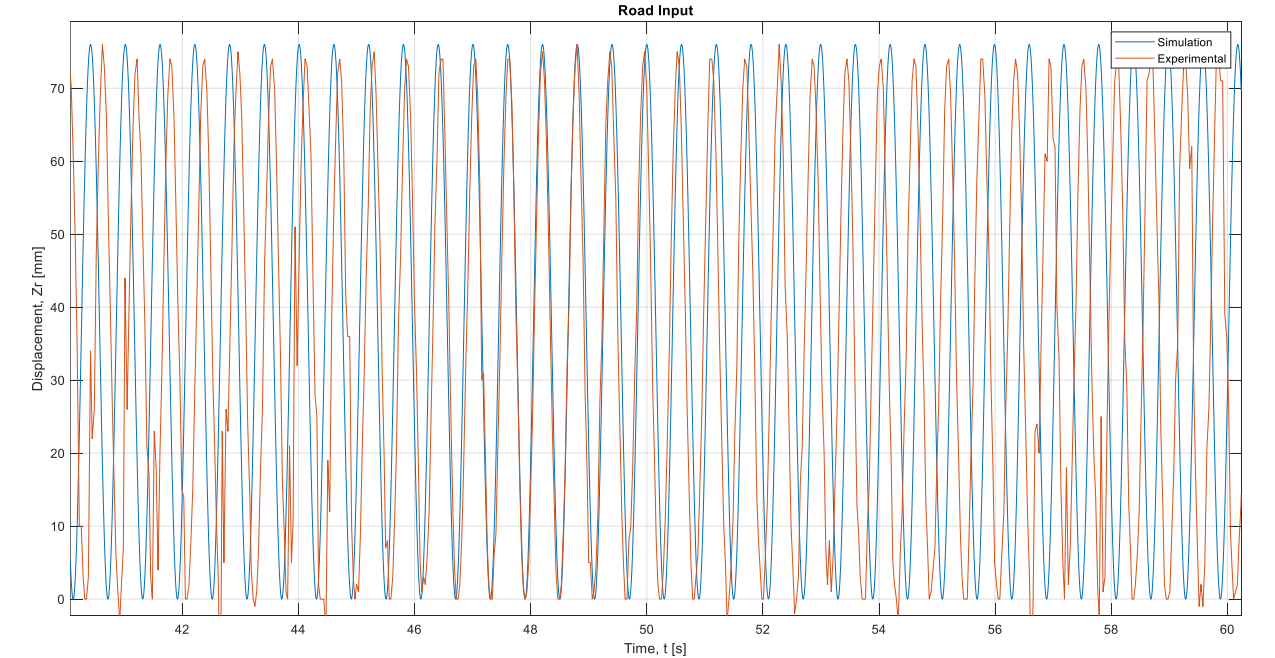
\includegraphics[width=0.99\linewidth]{figures/1.67 RI.png}
	\caption{Road Input Comparison at 1.670 [Hz]}
	\label{fig:Road Input Comparison at 1.670}
\end{figure}


\section{Unsprung mass Displacement Comparison}
\begin{itemize}
	\item 0.309 [Hz]
\end{itemize}
\begin{figure}[H]
	\centering
	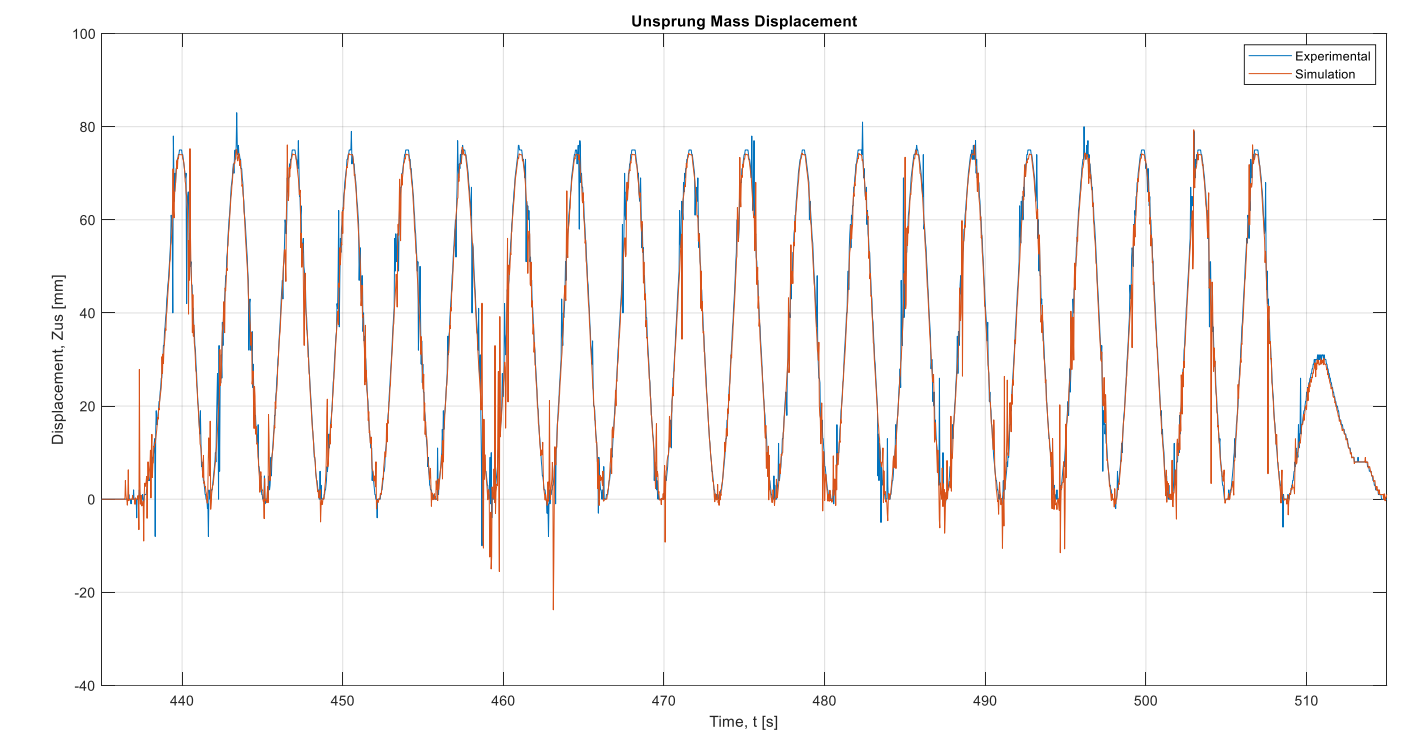
\includegraphics[width=0.9\linewidth]{figures/0.309 Us.png}
	\caption{Unsprung mass Displacement Comparison at 0.309 [Hz]}
	\label{fig:Unsprung mass Displacement Comparison at 0.309}
\end{figure}

\begin{itemize}
	\item 0.817 [Hz]
\end{itemize}
\begin{figure}[H]
	\centering
	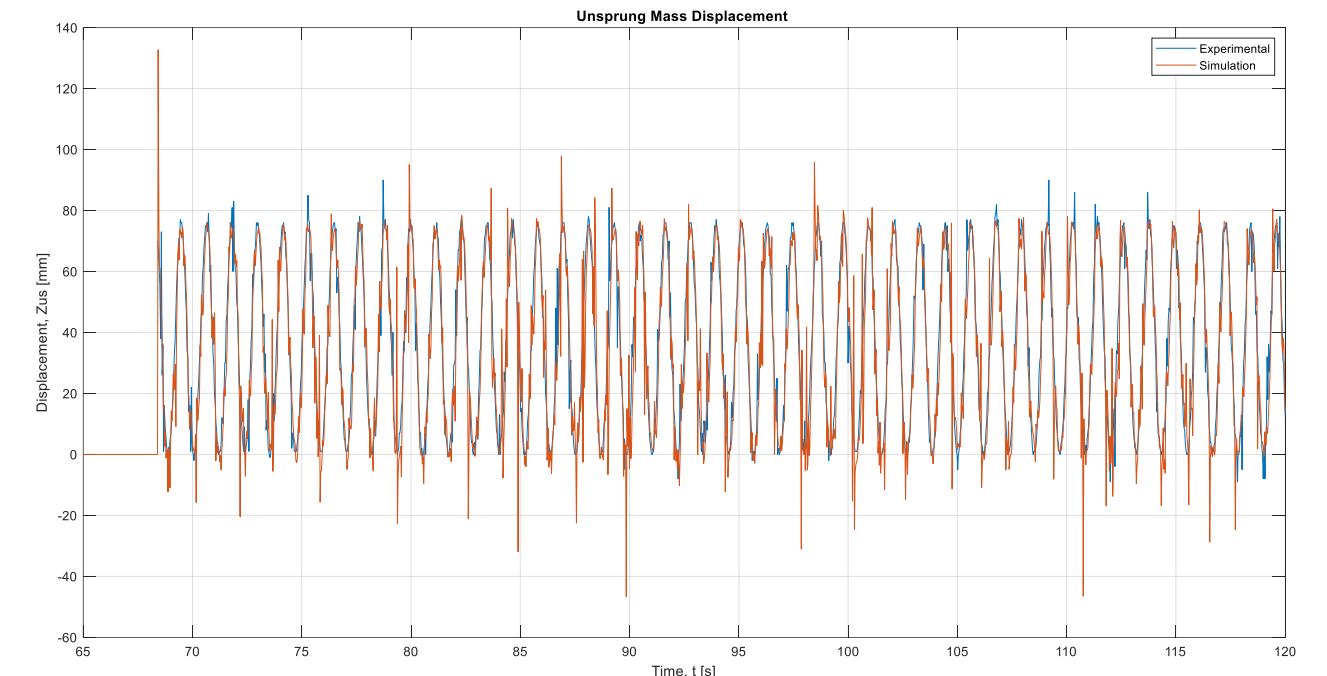
\includegraphics[width=0.99\linewidth]{figures/0.817 Us.png}
	\caption{Unsprung mass Displacement Comparison at 0.817 [Hz]}
	\label{fig:Unsprung mass Displacement Comparison at 0.817}
\end{figure}


\begin{itemize}
	\item 1.670 [Hz]
\end{itemize}
\begin{figure}[H]
	\centering
	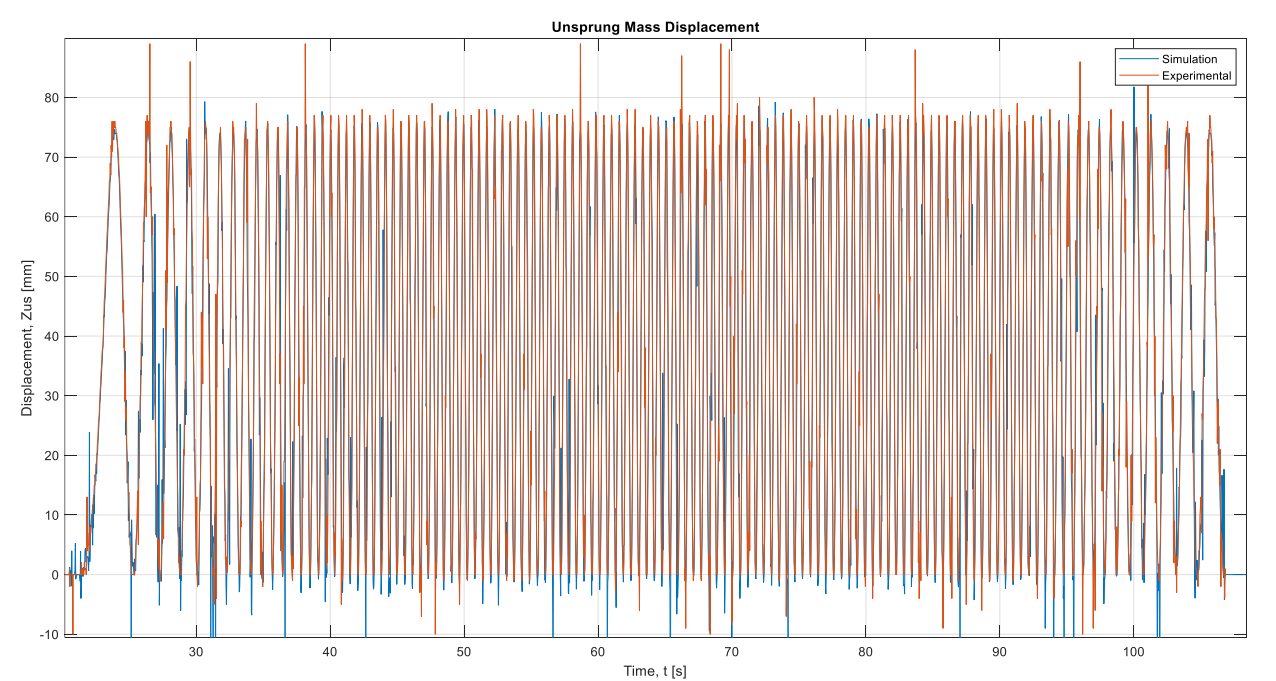
\includegraphics[width=0.99\linewidth]{figures/1.67 Us.png}
	\caption{Unsprung mass Displacement at 1.670 [Hz]}
	\label{fig:Unsprung mass Displacement Comparison at 1.670}
\end{figure}

\section{Sprung mass Displacement Comparison}
\begin{itemize}
	\item 0.309 [Hz]
\end{itemize}
\begin{figure}[H]
	\centering
	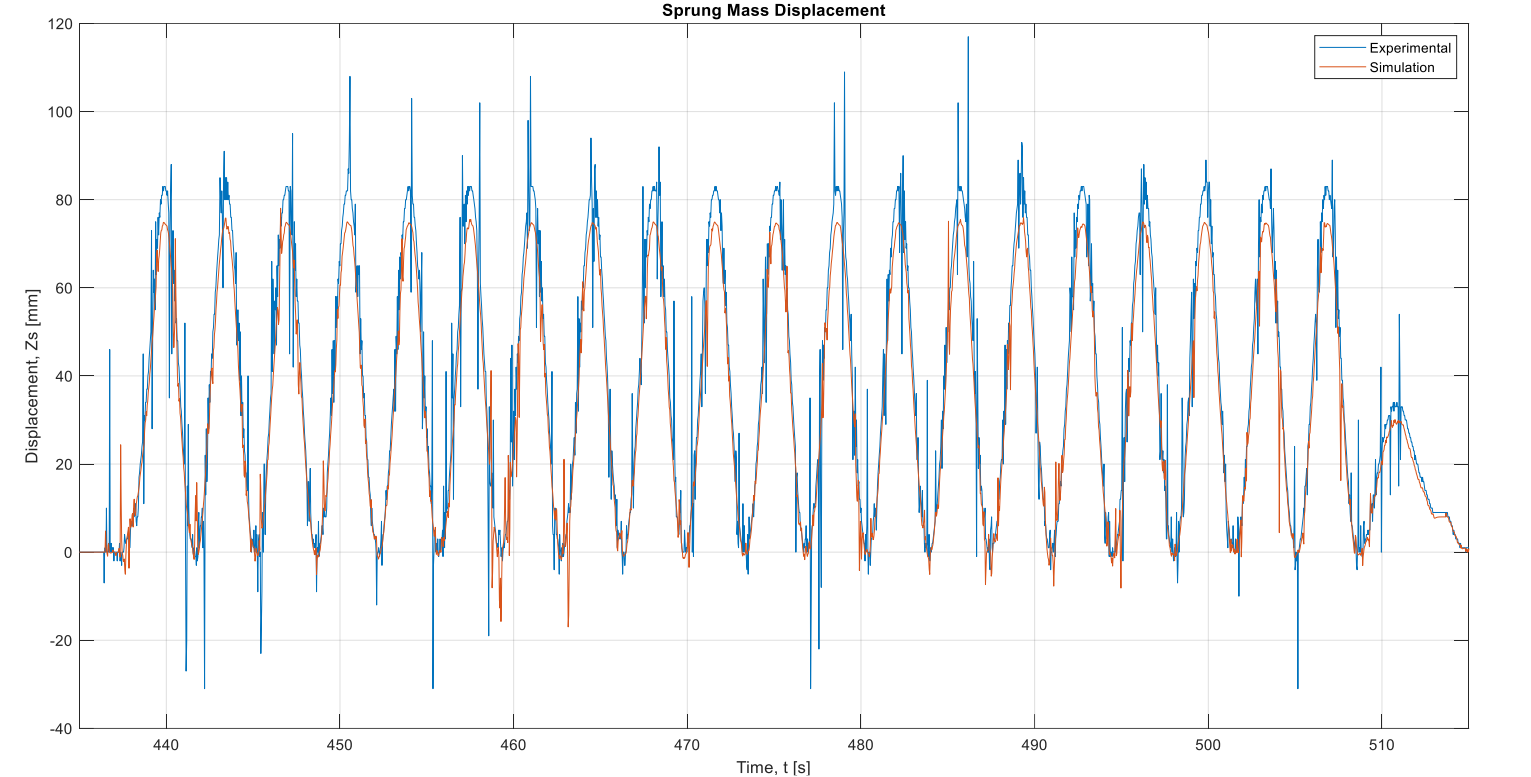
\includegraphics[width=0.9\linewidth]{figures/0.309 S.png}
	\caption{Sprung mass Displacement Comparison at 0.309 [Hz]}
	\label{fig:Sprung mass Displacement Comparison at 0.309}
\end{figure}

\begin{itemize}
	\item 0.817 [Hz]
\end{itemize}
\begin{figure}[H]
	\centering
	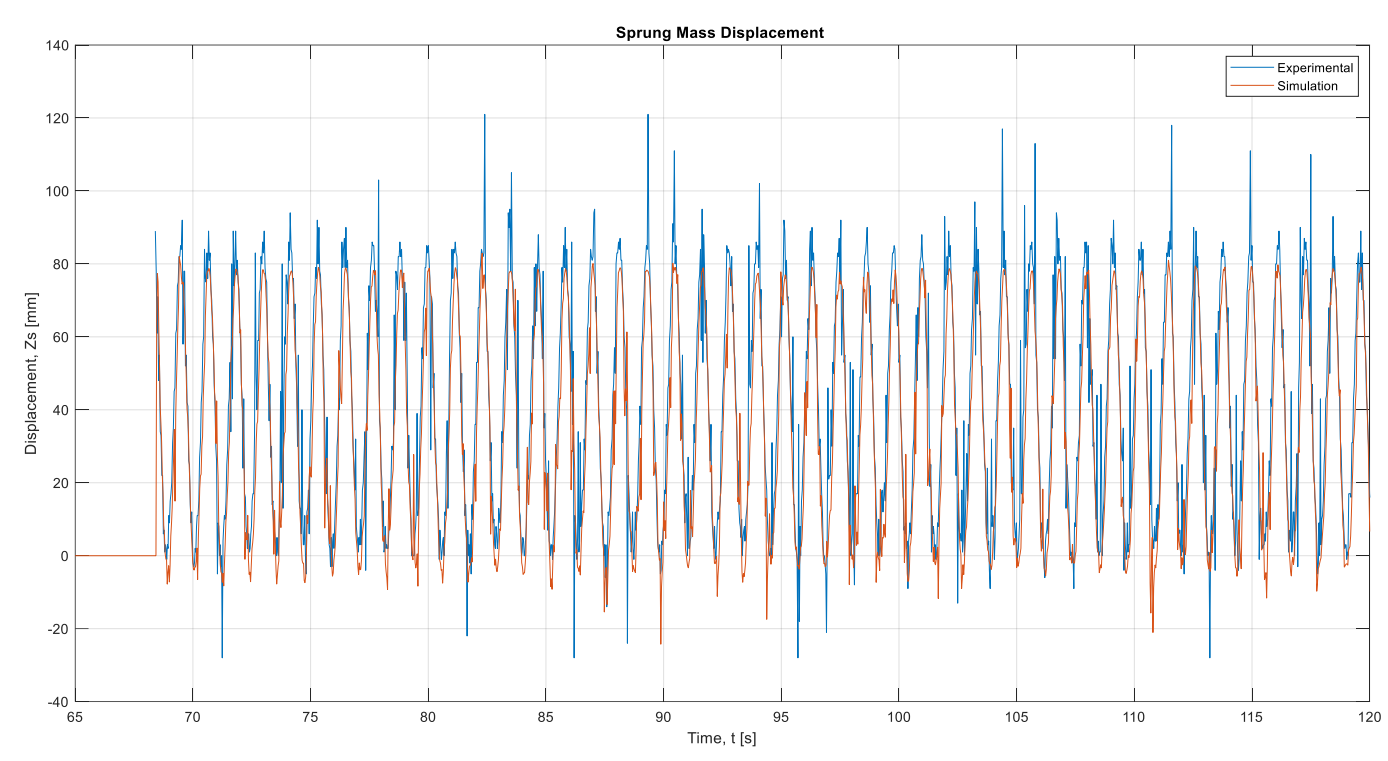
\includegraphics[width=0.99\linewidth]{figures/0.817 S.png}
	\caption{Sprung mass Displacement Comparison at 0.817 [Hz]}
	\label{fig:Sprung mass Displacement Comparison at 0.817}
\end{figure}

\begin{itemize}
	\item 1.670 [Hz]
\end{itemize}
\begin{figure}[H]
	\centering
	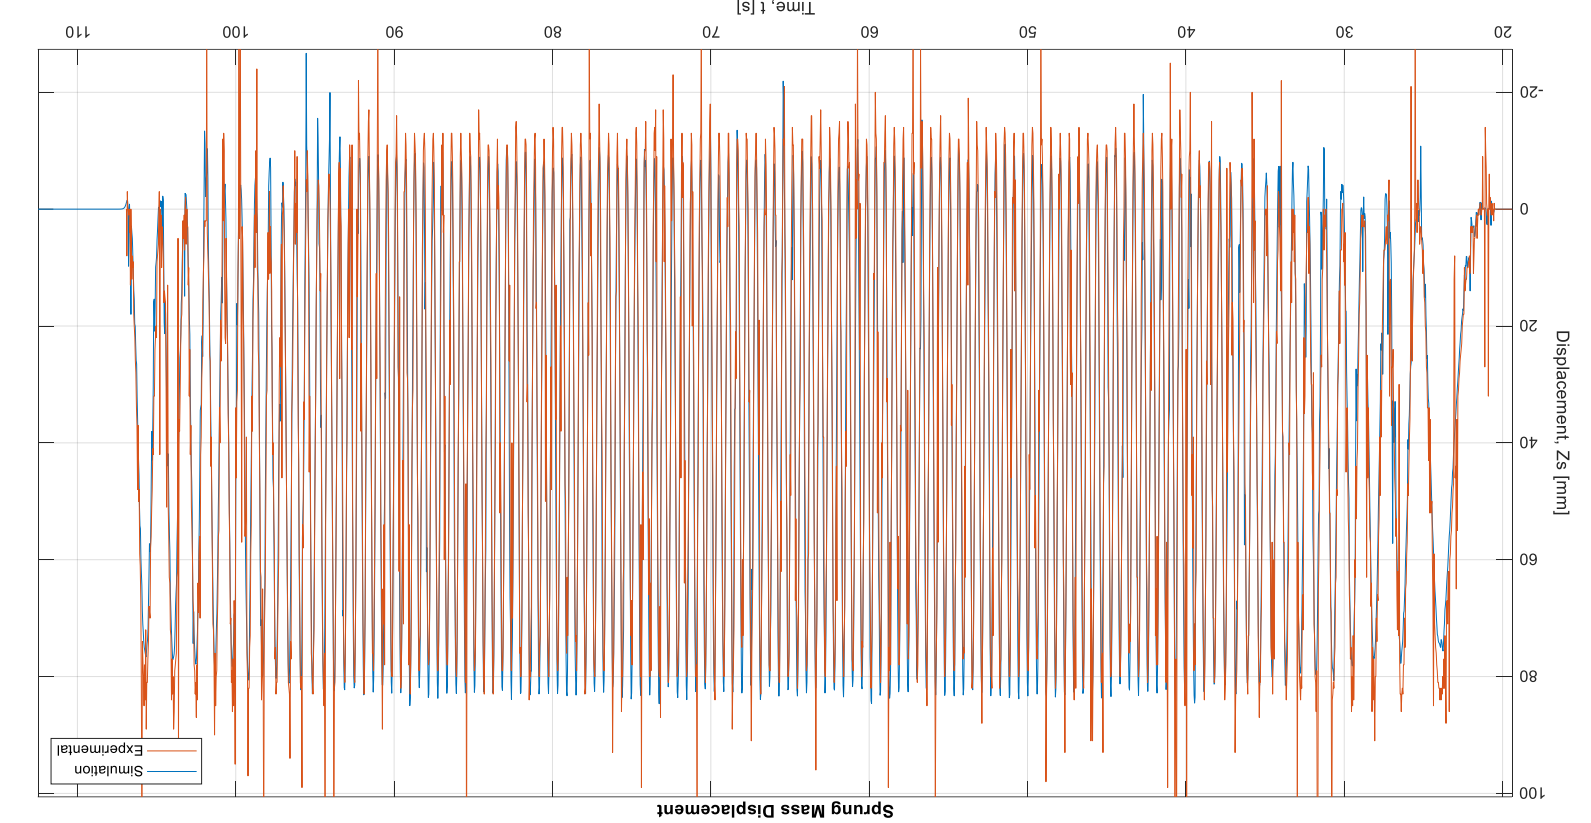
\includegraphics[width=0.99\linewidth]{figures/1.67 S.png}
	\caption{Sprung mass Displacement at 1.670 [Hz]}
	\label{fig:Sprung mass Displacement Comparison at 1.670}
\end{figure}

\section{Conslusion}

As shown in the results above, the simulation model results is very close to the experimental results in the Road Input, Unsprung mass displacement and sprung mass displacement.
\newline
So, the simulation model is valid.
\fi

\chapter{Modern Control Techniques}
\section{Conclusion}
This study demonstrated that the sliding mode controller (SMC) outperforms the linear quadratic regulator (LQR). As expected from the literature, the LQR provides an improvement over passive control but lacks the robustness and adaptability of advanced control strategies. While reinforcement learning (RL) has shown promise in recent studies, a direct comparison was not feasible due to the extensive training and tuning required. Overall, SMC proves to be a more effective solution for achieving superior performance and robustness in this application.


\section{Future Work}
In the next semester we  will implement, and experimentally validate a Hardware-in-the-Loop (HIL) results for the active suspension system on a quarter-car model test rig. This will involve:

\begin{itemize}
	\item Integrating the previously developed simulation models with the real quarter-car model test rig.
	\item Developing and implementing data acquisition and the simulated control algorithms within the HIL environment.
	\item Conducting rigorous experimental testing to compare the performance of the simulated and real-time implementations of the active suspension system under various road excitations.
	\item Analyzing the experimental results to assess the accuracy and effectiveness of the control algorithms, identify any difference between the simulated and real-world behavior of the quarter-car model, and quantify the achieved ride comfort and handling improvements.
	\item Investigating and mitigating the effects of sensor noise and actuator limitations on the system's performance within the context of the quarter-car model test rig.
	\item Refining the control algorithms based on the experimental findings to optimize the suspension system's ride comfort, handling, and road holding capabilities on the quarter-car model.
\end{itemize}

\chapter{Results and Conclusion}









\iffalse
\section{Conclusion}
In this section we are going to conclude the analysis and our study. We will remind you what was in this report.
\begin{itemize}
	\item Firstly, we introduced the study with the automobile's history including overview on the car as one of the complicated machines, then the history of transformation from the horses to the cars in means of reliability and comfortability in the road transportation. Then we talked about the vehicle suspension system components and its evolution and improvement. Also, the debit between the ride quality and vehicle handling was demonstrated.
	\item To get into studying and improving the vehicle suspension system, we investigated in the previous literatures talking about the motivation and purposes to push the automotive industry and researchers to enhance the passive suspension system.
	\item Then we provided the experimental work. In one hand, the mechanical part including the preparation of the real physical model, the experiments for passive suspension parameters such as control arm, wheel and tire assembly, and setup frame moment inertia. Then we got the wheel reaction and sprung mass. In the other hand, the electronic part including the sensors used with their specification and wiring to reveal the data.
	\item The mathematical model of passive suspension system section was talking about the three model dynamic models:
	\begin{itemize}
		\item Two DOF quarter-car models.
		\item Four DOF half-car models.
		\item Seven DOF full- car models
	\end{itemize}
	
	These are commonly used models for the theoretical analysis and design of suspension systems.
	
	The state space representation was the mathematical model used in our model representation. It was used because it provides a concise and systematic way to represent the evolution of a system over time.
	
	The conventional two DOF quarter-car model was modified to include the inertia effects to simulate our real model and setup.
	
	After that, the result of dynamic response analysis and comparing between the simplified (conventional) and Inertial Quarter-car Suspension model. The analysis concluded that Sprung and Unsprung acceleration curves of the inertial model exceed those of the simplified model by 14.3\% and 3.8\%, respectively.
	
	A bump Profile is described as a road disturbance. These bumps simulate irregularities or variations in the road surface that can impact a vehicle's suspension system.
	
	The inputs to our system were different road input profiles as follows:
	\begin{itemize}
		\item Sinusoidal Bump
		\item Trapezoidal Bump
		\item Parabolic Bump
	\end{itemize}
	Then the results in terms of displacement, acceleration, suspension travel and tire deflection were demonstrated with different road input profiles and with including the tire radius effect.
	
	\item In the validation of simulation model section was comparing the data revealed from the real model with the simulation model data and was demonstrated the difference between them and the purposes that led to those differences
\end{itemize}

\section{Next Semester Work}
The study to this point not terminated but was very promising to go with improvement and enhancing such as:
\begin{itemize}
	\item Including each effect of the suspension elements in the simulation model.
	\item Including a parametric study and show the effect of changing the values of these suspension parameters.
\end{itemize}
Once this study and additional investigation is done, will let us to get into the upgrading to active suspension and the modification of our model to adapt the installation of the additional elements to enhance the system response.

\newpage

\fi


\appendix
\chapter{Appendices}
\section{Appendix 1 }
The following are some characteristics of springs:

Suspension Rate or Stiffness (K) is one of the characteristics that mean that the force needed to compress or extend a suspension spring by a specific amount of distance is known as the spring rate, also known as stiffness. Newtons per millimeter (N/m) are the common units of measurement.

Increased spring rates give the suspension more stiffness, which enhances responsiveness and handling. But too stiff of springs can make for a rough ride. And this will be well discussed in the suspension system conflicts section. \cite{trzesniowski2023suspension}

\section{Appendix 2}
	\begin{itemize}
	
	\item \textbf{Vibration Isolation:} This term means the response of the sprung mass (all components directly supported by the suspension system. Vehicle body and passenger passengers) to the various excitation types from the road. In most cases, \textbf{the transmissibility ratio} (transfer function) is used for evaluating a linear suspension system's vibration isolation ability.
	
	\begin{equation}
		TR=\frac{Z_\text{s}}{Z_\text{0}}
	\end{equation}
	where:
	\begin{itemize}[label=\textbullet]
		\item TR is the transmissibility ratio of the suspension system.
		\item $Z_\text{s}$ is the sprung mass displacement.
		\item $Z_\text{0}$ is the road excitation displacement.
	\end{itemize}
	
	\item \textbf{Suspension Travel (ST):} This means the deflection of the suspension spring or the relative displacement between the sprung mass (Car Body) and unsprung mass (components that are not supported by the suspension system i.e. The wheels and tires).
	\begin{equation}
		ST=\frac{Z_\text{us}-Z_\text{s}}{Z_\text{0}}
	\end{equation}
	where:
	\begin{itemize}[label=\textbullet]
		\item $ST$	is the suspension travel relative to road excitation displacement.
		\item $Z_\text{us}$	is the unsprung mass displacement.
		\item $Z_\text{s}$ is the sprung mass displacement.
	\end{itemize}
	\item \textbf{Roadholding:} The usual force acting between the tire and the road varies as the vehicle system vibrates on the road. The roadholding capabilities, handling, and performance of the vehicle are all influenced by tire vibration, since the cornering force, tractive effort, and braking effort generated by the tire are all associated with the tire's normal load. The displacement of the unsprung mass with respect to the road surface can be used to depict the normal force between the tire and the road during vibration. \textbf{The dynamic tire deflection} is used as a measurable term for evaluating the suspension performance characteristic as this formula:
	\begin{equation}
		DTD=\frac{Z_\text{0}-Z_\text{us}}{Z_\text{0}}
	\end{equation}
	where:
	\begin{itemize}[label=\textbullet]
		\item DTD is the dynamic tire deflection.
		\item $Z_\text{0}$ is the road excitation displacement.
		\item $Z_\text{us}$	is the unsprung mass displacement.
	\end{itemize}
\end{itemize}

\section{Appendix 3}
As an illustration figures \ref{fig:1.1} and \ref{fig:1.2} shows the tradeoffs in suspension design, the response of a passive suspension system at different suspension parameters implemented by suspension mathematical modeling using MATLAB software, it resulted:

A stiffer suspension behavior is required to enhance tire contact with the road-dynamic tire deflection-and the vehicle's dynamic behavior during braking and turning, whereas a softer suspension behavior is required to increase vehicle vibration isolation and enhance passenger comfort. \cite{east2021experimental}

\begin{figure}[H]
\centering
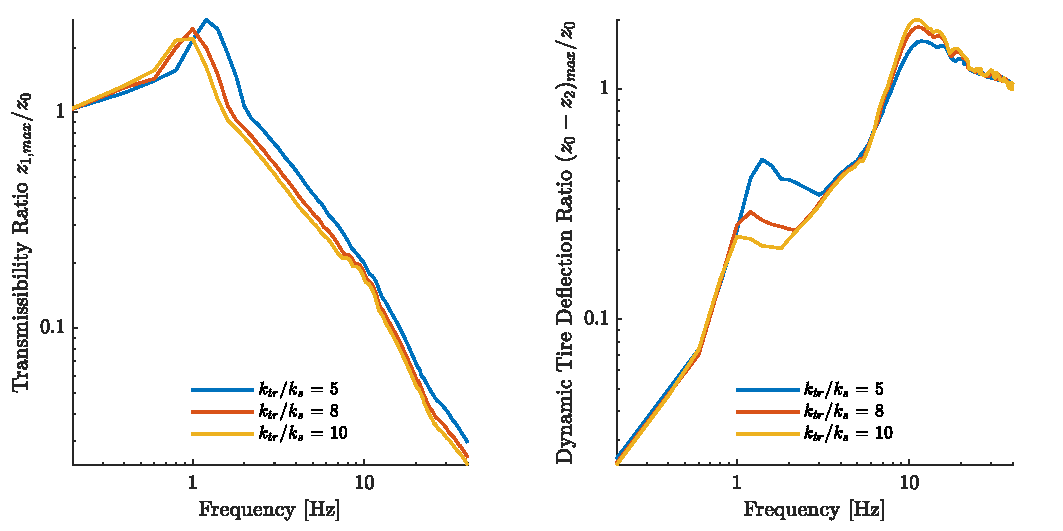
\includegraphics[width=\textwidth]{Stiffness Ratio.pdf}
\caption{Transmissibility ratio (left) and Dynamic Tire Deflection (right) as a function of frequency for the sprung mass of a suspension system with different ratios of tire stiffness to suspension spring stiffness}
\label{fig:1.1}
\end{figure}

\textbf{On the other hand}, As shown in figures 1.3 and 1.4, talking about the damping ratio ($\zeta$), the smaller damping ratio is required to high vibration isolation and good ride quality (lower transmissibility ratio), the natural frequency of the sprung mass or close to the natural frequency of the unsprung mass, to maintain good roadholding capability, higher damping is required. \cite{wong2001theory}

\begin{figure}[H]
\centering
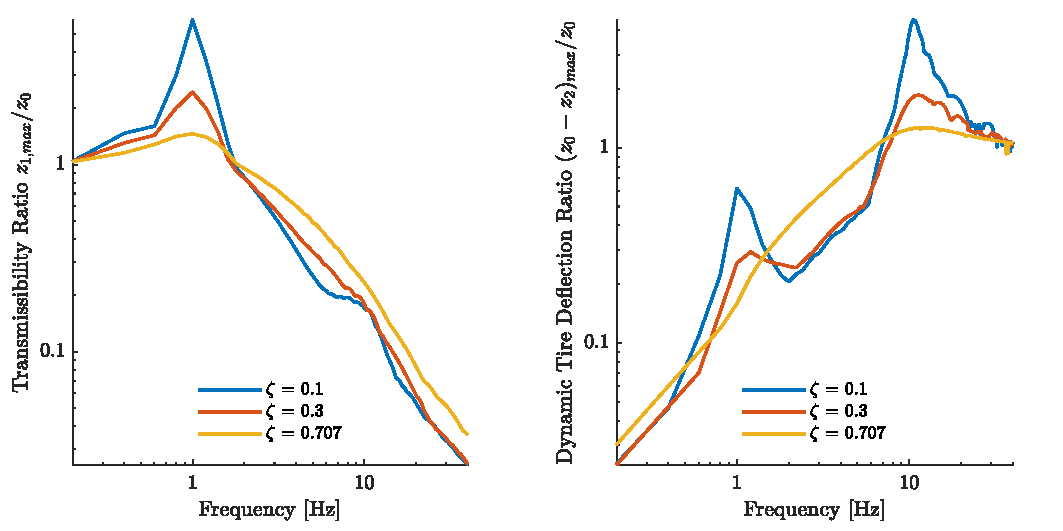
\includegraphics[width=\textwidth]{Damping Ratio.pdf}
\caption{Transmissibility ratio (left) and Dynamic Tire Deflection (right) as a function of frequency for the sprung mass of a suspension system with different damping ratios.}
\label{fig:1.2}
\end{figure}

And this presents a very difficult challenge for the designers, who have to make some compromises to strike a balance barely that is appropriate for maintaining the luxurious and safe driving experience of the vehicle. Furthermore, these compromises affect overall driving experience or vehicle safety and handling. \cite{east2021experimental}

For talking about \textbf{compromises in better overall driving experience} or ride quality, the International Standard IS0 2631 provides an extensive basis for characterizing human tolerance to whole-body vibration. The guide provides three different limits for whole-body vibration: Exposure limit, fatigue, and Reduced comfort. And is suggested for use in industry and in the evaluation of vibratory environments in transport vehicles. And may be considered as guiding for designers in determining the trade-off limits between vehicle road holding and ride comfort reduction. \cite{oborne1983whole}

\textbf{Exposure limits:} which, unless there is a specific reason, should not be exceeded in order to preserve safety (or health).

\textbf{Fatigue or decreased proficiency boundaries:} They pertain to maintaining operational efficiency and are applicable to jobs like operating a tractor or a road vehicle (driving for many hours).

\textbf{Reduced comfort boundaries:} which deal with maintaining comfort in transportation vehicles and are associated with activities like eating, writing, and reading in a car. \cite{east2021experimental}, \cite{oborne1983whole}\\
\textbf{-Road Holding}\\
On the other hand, talking about \textbf{compromises in road holding}, when a vehicle travels on the road, many factors may affect the vehicle holding cause instability. Among the problems related to car instability, reduced road holding in steering or braking or roll over condition, and this is the most dangerous phenomenon. All passengers and goods on board are threatened when the vehicle get instability in the road. Even the life of the car user may not be guaranteed once the instability accident occurs. Developed countries have better road conditions so that cars can travel at very high speeds. But this is not enough to avoid reduced road holding in all driving conditions. \cite{nguyen2023establishing}

In general luxury cars typically have suspension systems that prioritize comfort over handling dynamics, which may cause the car to lose stability when braking and turning at specific high speeds. As a result, these vehicles offer a comfortable ride and are adept at swallowing bumps, but handling and control are compromised. However, the suspension of sports cars is usually designed with a focus on handling, meaning that while improving the road holding and stability, ride quality and comfort are compromised. Therefore, there is a trade-off between comfort and vehicle control when using passive suspension systems (PSS). \cite{kuber2014modelling}


\bibliographystyle{unsrtnat}
\bibliography{ref}


\end{document}

